
\documentclass[xcolor=dvipsnames]{beamer}  % for hardcopy add 'trans'

\mode<presentation>
{
  \usetheme{Singapore}
  % or ...
  \setbeamercovered{transparent}
  % or whatever (possibly just delete it)
}

\usefonttheme{professionalfonts}
\usepackage[russian]{babel}
% or whatever
%\usepackage[latin1]{inputenc}
% or whatever
%\usepackage{times}
%\usepackage[T1]{fontenc}
% Or whatever. Note that the encoding and the font should match. If T1
% does not look nice, try deleting the line with the fontenc.

%%%%%%%%%%%%%%%%%%%%%% start my preamble %%%%%%%%%%%%%%%%%%%%%%


\addtobeamertemplate{navigation symbols}{}{%
    \usebeamerfont{footline}%
    \usebeamercolor[fg]{footline}%
    \hspace{1em}%
    \insertframenumber/\inserttotalframenumber
} 

\setbeamercolor{footline}{fg=blue}
\setbeamerfont{footline}{series=\bfseries}


%\usepackage{epsfig}
\usepackage{graphicx}
\graphicspath{{./figs_code/}}

\usepackage{amsmath, amssymb, amsthm}

\usepackage{fancyvrb}

\usepackage{tikz}
\usetikzlibrary{arrows}
\usetikzlibrary{calc}
\usetikzlibrary{intersections}
\usetikzlibrary{decorations}
\usepackage{pgf}
\usepackage{pgfplots}
\pgfplotsset{compat=1.13}

\usepackage{graphviz}
 
\usepackage{verbatim}


\usepackage{algorithmicx,algpseudocode}


%font
\usepackage{mathpazo}
%\usepackage[usenames, dvipsnames]{color}

%\usepackage[linesnumbered, ruled, lined]{algorithm2e}

\usepackage{xr}
\externaldocument[ET-]{et}


\newcommand*{\theorembreak}{\usebeamertemplate{theorem end}\framebreak\usebeamertemplate{theorem begin}}

\newcommand{\newtopic}[1]{\textcolor{Green}{\Large \bf #1}}
\newcommand{\navy}[1]{\textcolor{Blue}{\bf #1}}
\newcommand{\navymth}[1]{\textcolor{Blue}{#1}}
\newcommand{\red}[1]{\textcolor{red}{#1}}


\definecolor{pale}{RGB}{235, 235, 235}
\definecolor{pale2}{RGB}{175,238,238}
\definecolor{turquois4}{RGB}{0,134,139}

% Typesetting code
\definecolor{bg}{rgb}{0.95,0.95,0.95}
\usepackage{minted}
\usemintedstyle{friendly}
\newminted{python}{mathescape,frame=lines,framesep=4mm,bgcolor=bg}
\newminted{ipython}{mathescape,frame=lines,framesep=4mm,bgcolor=bg}
\newminted{julia}{mathescape,frame=lines,framesep=4mm,bgcolor=bg}
\newminted{c}{mathescape,linenos=true}
\newminted{r}{mathescape,  frame=none, baselinestretch=1, framesep=2mm}
\renewcommand{\theFancyVerbLine}{\sffamily
    \textcolor[rgb]{0.5,0.5,1.0}{\scriptsize {\arabic{FancyVerbLine}}}}


\usepackage{stmaryrd}

\newcommand{\Fact}{\textcolor{Brown}{\bf Факт. }}
\newcommand{\Facts}{\textcolor{Brown}{\bf Факты }}
\newcommand{\keya}{\textcolor{turquois4}{\bf Ключевая идея. }}
\newcommand{\Factnodot}{\textcolor{Brown}{\bf Факт }}
\newcommand{\Eg}{\textcolor{ForestGreen}{Пример. }}
\newcommand{\Egs}{\textcolor{ForestGreen}{Примеры. }}
\newcommand{\Ex}{{\bf Ex. }}
\newcommand{\Thm}{\textcolor{Brown}{\bf Теорема. }}
\newcommand{\Prf}{\textcolor{turquois4}{\bf Доказательство. }}
\newcommand{\Ass}{\textcolor{turquois4}{\bf Допущение.}} 
\newcommand{\Lem}{\textcolor{Brown}{\bf Лемма. }}

%source code 



% cali
\usepackage{mathrsfs}
\usepackage{bbm}
\usepackage{subfigure}

\newcommand{\argmax}{\operatornamewithlimits{argmax}}
\newcommand{\argmin}{\operatornamewithlimits{argmin}}

\newcommand\T{{\mathpalette\raiseT\intercal}}
\newcommand\raiseT[2]{\raisebox{0.25ex}{$#1#2$}}

\DeclareMathOperator{\cl}{cl}
%\DeclareMathOperator{\argmax}{argmax}
\DeclareMathOperator{\interior}{int}
\DeclareMathOperator{\Prob}{Prob}
\DeclareMathOperator{\kernel}{ker}
\DeclareMathOperator{\diag}{diag}
\DeclareMathOperator{\sgn}{sgn}
\DeclareMathOperator{\determinant}{det}
\DeclareMathOperator{\trace}{trace}
\DeclareMathOperator{\Span}{span}
\DeclareMathOperator{\rank}{rank}
\DeclareMathOperator{\cov}{cov}
\DeclareMathOperator{\corr}{corr}
\DeclareMathOperator{\range}{rng}
\DeclareMathOperator{\var}{var}
\DeclareMathOperator{\mse}{mse}
\DeclareMathOperator{\se}{se}
\DeclareMathOperator{\row}{row}
\DeclareMathOperator{\col}{col}
\DeclareMathOperator{\dimension}{dim}
\DeclareMathOperator{\fracpart}{frac}
\DeclareMathOperator{\proj}{proj}
\DeclareMathOperator{\colspace}{colspace}

\providecommand{\inner}[1]{\left\langle{#1}\right\rangle}

% mics short cuts and symbols
% mics short cuts and symbols
\newcommand{\st}{\ensuremath{\ \mathrm{s.t.}\ }}
\newcommand{\setntn}[2]{ \{ #1 : #2 \} }
\newcommand{\cf}[1]{ \lstinline|#1| }
\newcommand{\otms}[1]{ \leftidx{^\circ}{#1}}

\newcommand{\fore}{\therefore \quad}
\newcommand{\tod}{\stackrel { d } {\to} }
\newcommand{\tow}{\stackrel { w } {\to} }
\newcommand{\toprob}{\stackrel { p } {\to} }
\newcommand{\toms}{\stackrel { ms } {\to} }
\newcommand{\eqdist}{\stackrel {\textrm{ \scriptsize{d} }} {=} }
\newcommand{\iidsim}{\stackrel {\textrm{ {\sc iid }}} {\sim} }
\newcommand{\1}{\mathbbm 1}
\newcommand{\dee}{\,{\rm d}}
\newcommand{\given}{\, | \,}
\newcommand{\la}{\langle}
\newcommand{\ra}{\rangle}

\renewcommand{\rho}{\varrho}

\newcommand{\htau}{ \hat \tau }
\newcommand{\hgamma}{ \hat \gamma }

\newcommand{\boldx}{ {\mathbf x} }
\newcommand{\boldu}{ {\mathbf u} }
\newcommand{\boldv}{ {\mathbf v} }
\newcommand{\boldw}{ {\mathbf w} }
\newcommand{\boldy}{ {\mathbf y} }
\newcommand{\boldb}{ {\mathbf b} }
\newcommand{\bolda}{ {\mathbf a} }
\newcommand{\boldc}{ {\mathbf c} }
\newcommand{\boldi}{ {\mathbf i} }
\newcommand{\bolde}{ {\mathbf e} }
\newcommand{\boldp}{ {\mathbf p} }
\newcommand{\boldq}{ {\mathbf q} }
\newcommand{\bolds}{ {\mathbf s} }
\newcommand{\boldt}{ {\mathbf t} }
\newcommand{\boldz}{ {\mathbf z} }

\newcommand{\boldzero}{ {\mathbf 0} }
\newcommand{\boldone}{ {\mathbf 1} }

\newcommand{\boldalpha}{ {\boldsymbol \alpha} }
\newcommand{\boldbeta}{ {\boldsymbol \beta} }
\newcommand{\boldgamma}{ {\boldsymbol \gamma} }
\newcommand{\boldtheta}{ {\boldsymbol \theta} }
\newcommand{\boldxi}{ {\boldsymbol \xi} }
\newcommand{\boldtau}{ {\boldsymbol \tau} }
\newcommand{\boldepsilon}{ {\boldsymbol \epsilon} }
\newcommand{\boldmu}{ {\boldsymbol \mu} }
\newcommand{\boldSigma}{ {\boldsymbol \Sigma} }
\newcommand{\boldOmega}{ {\boldsymbol \Omega} }
\newcommand{\boldPhi}{ {\boldsymbol \Phi} }
\newcommand{\boldLambda}{ {\boldsymbol \Lambda} }
\newcommand{\boldphi}{ {\boldsymbol \phi} }

\newcommand{\Sigmax}{ {\boldsymbol \Sigma_{\boldx}}}
\newcommand{\Sigmau}{ {\boldsymbol \Sigma_{\boldu}}}
\newcommand{\Sigmaxinv}{ {\boldsymbol \Sigma_{\boldx}^{-1}}}
\newcommand{\Sigmav}{ {\boldsymbol \Sigma_{\boldv \boldv}}}

\newcommand{\hboldx}{ \hat {\mathbf x} }
\newcommand{\hboldy}{ \hat {\mathbf y} }
\newcommand{\hboldb}{ \hat {\mathbf b} }
\newcommand{\hboldu}{ \hat {\mathbf u} }
\newcommand{\hboldtheta}{ \hat {\boldsymbol \theta} }
\newcommand{\hboldtau}{ \hat {\boldsymbol \tau} }
\newcommand{\hboldmu}{ \hat {\boldsymbol \mu} }
\newcommand{\hboldbeta}{ \hat {\boldsymbol \beta} }
\newcommand{\hboldgamma}{ \hat {\boldsymbol \gamma} }
\newcommand{\hboldSigma}{ \hat {\boldsymbol \Sigma} }

\newcommand{\boldA}{\mathbf A}
\newcommand{\boldB}{\mathbf B}
\newcommand{\boldC}{\mathbf C}
\newcommand{\boldD}{\mathbf D}
\newcommand{\boldI}{\mathbf I}
\newcommand{\boldL}{\mathbf L}
\newcommand{\boldM}{\mathbf M}
\newcommand{\boldP}{\mathbf P}
\newcommand{\boldQ}{\mathbf Q}
\newcommand{\boldR}{\mathbf R}
\newcommand{\boldX}{\mathbf X}
\newcommand{\boldU}{\mathbf U}
\newcommand{\boldV}{\mathbf V}
\newcommand{\boldW}{\mathbf W}
\newcommand{\boldY}{\mathbf Y}
\newcommand{\boldZ}{\mathbf Z}

\newcommand{\bSigmaX}{ {\boldsymbol \Sigma_{\hboldbeta}} }
\newcommand{\hbSigmaX}{ \mathbf{\hat \Sigma_{\hboldbeta}} }

\newcommand{\RR}{\mathbbm R}
\newcommand{\CC}{\mathbbm C}
\newcommand{\NN}{\mathbbm N}
\newcommand{\PP}{\mathbbm P}
\newcommand{\EE}{\mathbbm E \nobreak\hspace{.1em}}
\newcommand{\EEP}{\mathbbm E_P \nobreak\hspace{.1em}}
\newcommand{\ZZ}{\mathbbm Z}
\newcommand{\QQ}{\mathbbm Q}


\newcommand{\XX}{\mathcal X}

\newcommand{\aA}{\mathcal A}
\newcommand{\fF}{\mathscr F}
\newcommand{\bB}{\mathscr B}
\newcommand{\iI}{\mathscr I}
\newcommand{\rR}{\mathscr R}
\newcommand{\dD}{\mathcal D}
\newcommand{\lL}{\mathcal L}
\newcommand{\llL}{\mathcal{H}_{\ell}}
\newcommand{\gG}{\mathcal G}
\newcommand{\hH}{\mathcal H}
\newcommand{\nN}{\textrm{\sc n}}
\newcommand{\lN}{\textrm{\sc ln}}
\newcommand{\pP}{\mathscr P}
\newcommand{\qQ}{\mathscr Q}
\newcommand{\xX}{\mathcal X}

\newcommand{\ddD}{\mathscr D}


\newcommand{\R}{{\texttt R}}
\newcommand{\risk}{\mathcal R}
\newcommand{\Remp}{R_{{\rm emp}}}

\newcommand*\diff{\mathop{}\!\mathrm{d}}
\newcommand{\ess}{ \textrm{{\sc ess}} }
\newcommand{\tss}{ \textrm{{\sc tss}} }
\newcommand{\rss}{ \textrm{{\sc rss}} }
\newcommand{\rssr}{ \textrm{{\sc rssr}} }
\newcommand{\ussr}{ \textrm{{\sc ussr}} }
\newcommand{\zdata}{\mathbf{z}_{\mathcal D}}
\newcommand{\Pdata}{P_{\mathcal D}}
\newcommand{\Pdatatheta}{P^{\mathcal D}_{\theta}}
\newcommand{\Zdata}{Z_{\mathcal D}}


\newcommand{\e}[1]{\mathbbm{E}[{#1}]}
\newcommand{\p}[1]{\mathbbm{P}({#1})}

%\theoremstyle{plain}
%\newtheorem{axiom}{Axiom}[section]
%\newtheorem{theorem}{Theorem}[section]
%\newtheorem{corollary}{Corollary}[section]
%\newtheorem{lemma}{Lemma}[section]
%\newtheorem{proposition}{Proposition}[section]
%
%\theoremstyle{definition}
%\newtheorem{definition}{Definition}[section]
%\newtheorem{example}{Example}[section]
%\newtheorem{remark}{Remark}[section]
%\newtheorem{notation}{Notation}[section]
%\newtheorem{assumption}{Assumption}[section]
%\newtheorem{condition}{Condition}[section]
%\newtheorem{exercise}{Ex.}[section]
%\newtheorem{fact}{Fact}[section]

% Bibliography
\usepackage[authordate,uniquename=false,firstinits,backend=biber,maxcitenames=2]{biblatex-chicago}
\DeclareFieldFormat[article]{title}{#1}
\DeclareFieldFormat[inproceedings]{title}{#1}
\addbibresource{et_newbib.bib}
\renewcommand{\cite}{\textcite}



\setlength{\parskip}{1.5ex plus0.5ex minus0.5ex}


\setlength{\jot}{12pt} 










\title{Учебник по Эконометрике}

\subtitle
{Лекция 4: Моделирование зависимости}

\author{Джон Стачурски \\ \vspace{.5em} 
	\scriptsize Лекции: Акшай Шенкер \\ \vspace{.1em} 
	\scriptsize Перевел: Алексей Кедо}


\begin{document}

\begin{frame}
  \titlepage
\end{frame}

\section{Случайные векторы и матрицы}

\begin{frame}\frametitle{Случайный вектор}
    
    \vspace{2em}
    \navy{Случайный вектор} $\boldx$ в $\RR^N$ --- это
    функция из $\Omega$ в $\RR^N$ со следующим свойством 
    %
    \begin{equation*}
        \label{eq:dorvv}
        \setntn{\omega \in \Omega}{\boldx(\omega) \in B} \in \fF
        \quad \text{для всех } B \in \bB(\RR^N)
    \end{equation*}
    
    \vspace{1em}
    Мы можем также определить \navy{случайный вектор} $\boldx$ в $\RR^N$ как
    список из $N$ случайных переменных $(x_1, \ldots, x_N)$
\end{frame}

\begin{frame}
    
    \vspace{2em}
    Пишем случайные векторы в строки или столбцы по удобству
    
    \begin{itemize}
        \item во время умножения матриц случайные векторы по умолчанию 
        будут векторами-столбцами
    \end{itemize}
    
    \vspace{1em}
    \Eg
    Вспомните эксперимент с обезьяной с завязанными глазами
    
    Пространство элементарных событий --- это единичный диск $\Omega := \setntn{(h, v) 
    	\in \RR^2}{\| (h, v) \| \leq 1}$ и пространство событий --- это Борелевские множества в $\Omega$
    
    Если $\boldx$ --- the identity on $\Omega$, то он просто сообщает результат
    $(h,v)$ --- случайный вектор
\end{frame}

\begin{frame}

    \vspace{2em}
    \Eg
    Рассмотрим случайную выборку с перечислением доходов $y_n$ индивидов $n=1,\ldots,N$
    
    Вектор $(y_1, \ldots, y_N)$ который сообщает результат этой выборки, можно 
    рассматривать как случайный вектор в $\RR^N$
    
\end{frame}

\begin{frame}\frametitle{Измеримость} 

     \vspace{2em}
    Определение случайного вектора гарантирует, что $\{\boldx \in B\}$ ---
    определенное событие для каждого $B \in \bB(\RR^N)$
    
    \vspace{1em}
    Чтобы убедиться, что $\boldy = f(\boldx)$ --- случайный вектор:
    
    \begin{itemize}
        \item функция $f \colon \RR^N \to \RR^M$ должна удовлетворять 
        $f^{-1}(B) \in \bB(\RR^N)$ для всех $B \in \bB(\RR^M)$
    \end{itemize}

\end{frame}

\begin{frame}\frametitle{Ожидания}

    \vspace{2em}
    Ожидания определяются поэлементно
    
    \vspace{1em}
    Если $\boldx = (x_1, \ldots, x_N)$ --- случайный вектор 
    в $\RR^N$, то 
    %
    \begin{equation*}
        \EE \boldx
        = 
        \EE
        \left(
        \begin{array}{c}
            x_1 \\
            x_2 \\
            \vdots \\
            x_N
        \end{array}
        \right)
        :=
        \left(
        \begin{array}{c}
            \EE x_1 \\
            \EE x_2 \\
            \vdots \\
            \EE x_N
        \end{array}
        \right)
    \end{equation*}

\end{frame}

\begin{frame}\frametitle{Random Matrix}

    \vspace{2em}
    \navy{Случайная матрица} $\boldX$ размера $M \times N$ --- массив случайных величин 
    размера $M \times N$
    
    Его ожидание определяется как
    %
    \begin{equation*}
        \EE \boldX
        := 
        \begin{pmatrix}
            \EE x_{11} & \cdots & \EE x_{1N} \\
            \vdots &  & \vdots \\
            \EE x_{M1} & \cdots & \EE x_{MN}
        \end{pmatrix}
    \end{equation*}
    %
    
\end{frame}

\begin{frame}

    \vspace{2em}
    Из линейности ожиданий (факт ~\ref{ET-fa:exprop}):
    
    \Fact\eqref{ET-fa:lemc}
    Если $\boldX$ и $\boldY$ --- случайные матрицы или векторы, и $\boldA$ и
    $\boldB$ постоянны и согласованны, то
    %
    \begin{equation*}
        \EE [ \boldA \boldX + \boldB \boldY ]
            =  \boldA \EE [\boldX ] + \boldB \EE[\boldY]
    \end{equation*}
    %

\end{frame}

\begin{frame}\frametitle{Ковариационная матрица}

    \vspace{2em}
    \navy{Ковариационная матрица} случайного вектора $\boldx$ в $\RR^N$ с 
    $\boldmu := \EE \boldx$ является матрицей размера $N \times N$ 
    %
    \begin{equation*}
        \label{eq:vcd1}
        \var [\boldx] := \EE [ (\boldx - \boldmu) (\boldx - \boldmu)^\T]
    \end{equation*}
    %
    Расширяем:
    %
    \small
    \begin{equation*}
        \var [\boldx]
        = 
        \begin{pmatrix}
            \EE [(x_1 - \mu_1)(x_1 - \mu_1)]
                & \cdots & \EE [(x_1 - \mu_1)(x_N - \mu_N)] \\
            \vdots & & \vdots \\
            \EE [(x_N - \mu_N)(x_1 - \mu_1)]  
                & \cdots & \EE [(x_N - \mu_N)(x_N - \mu_N)] \\
        \end{pmatrix}
    \end{equation*}
    \normalsize
    
    $j,k$-ый является скалярной ковариацией между $x_j$ и $x_k$, и
    главная диагональ содержит дисперсию каждого $x_n$
    
\end{frame}

\begin{frame}

    \vspace{2em}
    \Fact
    Для любого случайного вектор $\boldx$ с $\EE[ \boldx^\T\boldx ] < \infty$,
    %
    \begin{enumerate}
        \item $\var [\boldx]$ существует и неотрицательно определена,
        \item $\var[\boldx] = \EE [\boldx \boldx^\T] - \boldmu \boldmu^\T$,
            и
        \item $\var[\boldA \boldx + \boldb] = \boldA \var[\boldx] \boldA^\T$
            \;\; (для любых постоянных и согласованных $\boldA, \boldb$).
    \end{enumerate}
    
\end{frame}


\begin{frame}

    \vspace{2em}
    \navy{Кросс-ковариация} между случайными векторами $\boldx$ и
    $\boldy$ определяется как 
    %
    \begin{equation*}
        \cov [\boldx, \boldy]
        := \EE [ (\boldx - \EE [\boldx]) (\boldy - \EE [\boldy])^\T]
    \end{equation*}
    %
    Очевидно, $\var[\boldx] = \cov[\boldx, \boldx]$
        
    \vspace{1em}
    \Fact\eqref{ET-fa:eoqf}
        Если $\boldz$ --- случайный вектор в $\RR^N$, удовлетворяющий $\EE[\boldz
        \boldz^\T] = \boldI$ и $\boldA$ любая постоянная матрица размера $N \times N$, то 
        %
        \begin{equation*}
            \EE[\boldz^\T \boldA \boldz] = \trace \boldA
        \end{equation*}
        %
    Доказательство --- решенное упражнение (смотрите упр.~\ref{ET-ex:eoqf})
    
\end{frame}

\begin{frame}\frametitle{Совместные распределения}

    \vspace{2em}
    \navy{Распределение} или \navy{закон} $P$ в $\RR^N$ --- вероятностная мера
    Борелевских множеств $\bB(\RR^N)$
    
    \vspace{1em}    
    По определению, оно удовлетворяет
    $P(\RR^N) = 1$ и $P(\cup_{n=1}^{\infty} B_n) = \sum_{n=1}^\infty
    P(B_n)$ для любых непересекающихся последовательностей $\{B_n\}$ в $\bB(\RR^N)$
    
\end{frame}

\begin{frame}

    \vspace{2em}
    \vspace{2em}
    \begin{figure}
    
       \begin{center}
        \scalebox{.4}{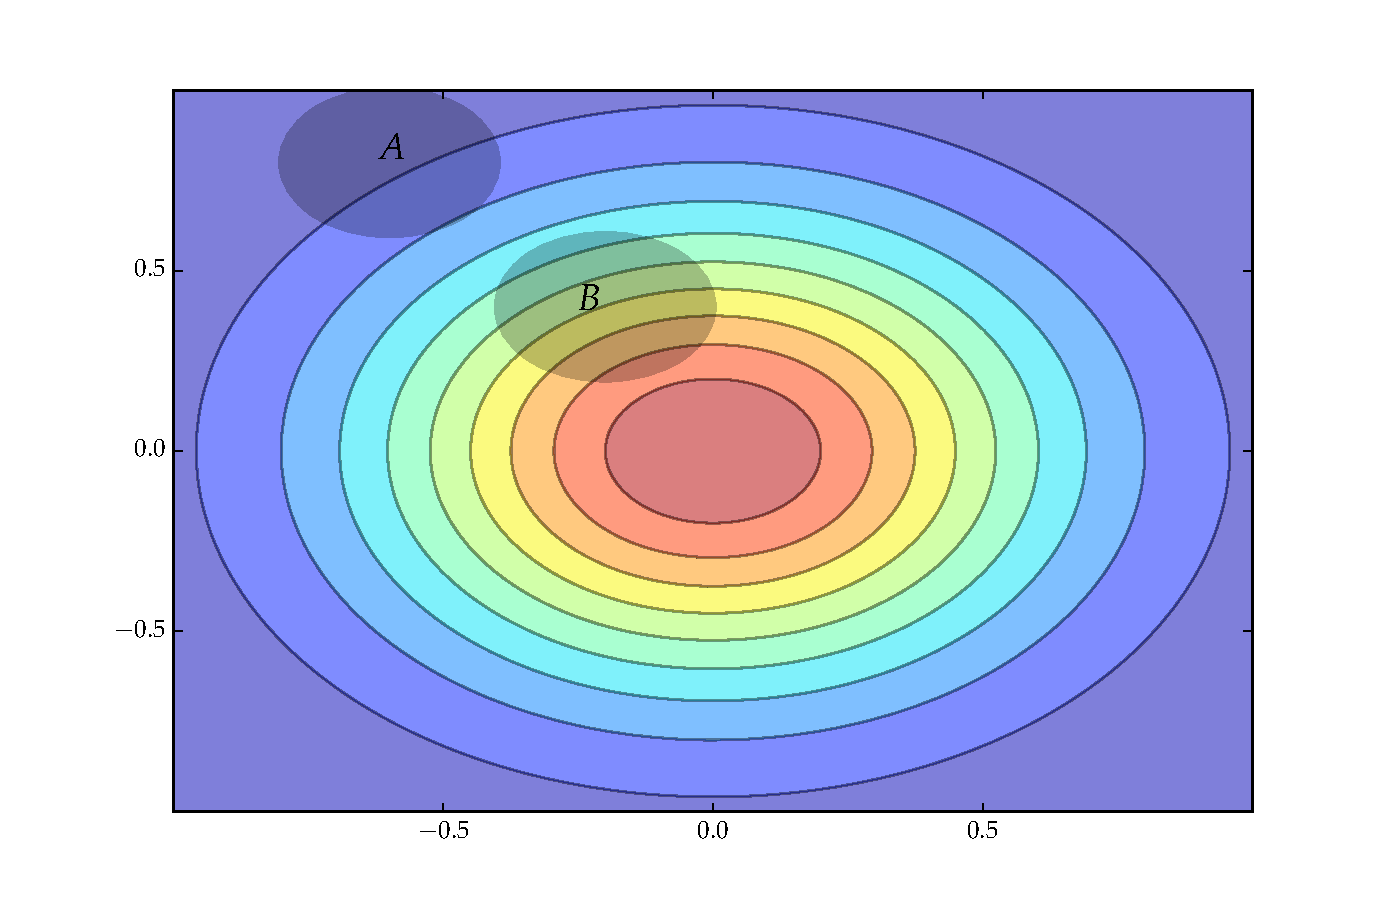
\includegraphics[trim={0 0em 0 2em}, clip]{gaussian_example.pdf}}
        \caption{\label{f:gaussian_example} Пример распределения и события $A$ и $B$}
       \end{center}
    \end{figure}  

\end{frame}



\begin{frame}

    \vspace{2em}
    Любое распределение $P$ в $\RR^N$ характеризуется функцией 
    %
    \begin{equation*}
    \label{eq:ntf2}
    F(\bolds) :=
    F(s_1, \ldots, s_N) 
    := P \left( \times_{n=1}^N (-\infty, s_n] \right)
    \qquad (\bolds \in \RR^N)
    \end{equation*}
    
    Функция $F$ --- \navy{функция совместного распределения},
    которая является функцией $F \colon \RR^N \to [0, 1]$ со следующими свойствами
    %
    \begin{enumerate}
            \label{enum:mcdf}
        \item непрерывна справа по каждому из своих аргументов,
        \item возрастает по каждому из своих аргументов, и 
        \item удовлетворяет
            %
            \begin{equation*}
                F(\bolds_j) \to 1 \text{ при }
                \bolds_j \to \infty 
                \quad 
            \end{equation*}
            \begin{equation*}
            \text{и} \quad
                F(s_1, \dots, s_{nj}, \dots, s_N) \to 0
                \text{ при }
                s_{nj} \to -\infty
            \end{equation*}
    \end{enumerate}
    
\end{frame}

\begin{frame}

    \vspace{2em}
     Распределение $P$ в $\RR^N$:
     %
     \begin{itemize}
         \item \navy{дискретно}, если $P$ имеет носитель распределения в счетном подпространстве $\RR^N$
         \item \navy{абсолютно непрерывно}, если $P(B) = 0$ всюду, где $B$ 
         имеет меру Лебега равную нулю
     \end{itemize}

\end{frame}

\begin{frame}
    
    \vspace{2em}
    Опять же, абсолютная непрерывность необходима и достаточна для существования 
    функции плотности:
    
    \begin{equation*}
    \label{eq:drbd3}
    P(B) = \int_B p(\bolds) \, \diff  \bolds
    \qquad \text{для всех } B \in \bB(\RR^N)
    \end{equation*}
    
    \vspace{2em}
    справа --- многомерный интеграл, который мы можем записать как
    %
    \begin{equation*}
        \label{eq:defjd0}
        \int_{-\infty}^{\infty}
            \cdots
            \int_{-\infty}^{\infty} 
            \1_B (s_1,\ldots,s_N)
            p(s_1,\ldots,s_N) 
            \diff s_1 \cdots \diff s_N
    \end{equation*}
    
    Если $p$ --- любая функция плотности в $\RR^N$, то вышенаписанное 
    определяет распределение
    
\end{frame}

\begin{frame}

    \vspace{2em}
    \Eg\label{eg:mnden}
    \navy{Многомерное нормальное распределение} или \navy{многомерное распределение Гаусса} 
    в $\RR^N$ --- функция $p$ вида
    %
    \begin{equation*}
        \label{eq:mnormden}
        p(\bolds) = (2 \pi)^{-N/2} \det(\boldSigma)^{-1/2} 
        \exp \left\{ 
            - \frac{1}{2} (\bolds - \boldmu)^\T \boldSigma^{-1} (\bolds - \boldmu) 
        \right\}
    \end{equation*}
    %
    где $\boldmu$ --- любой вектор размера $N \times 1$ и $\boldSigma$ --- положительно
    определенная матрица размера $N \times N$ 
    
    Представим это распределение как $\nN(\boldmu, \boldSigma)$
    
    \vspace{1em}
    Случай $\nN(\boldzero, \boldI)$ называется \navy{многомерным стандартным 
    	нормальным распределением}
    
\end{frame}

\begin{frame}

    \vspace{2em}
    \begin{figure}
    
   \centering
   \scalebox{.42}{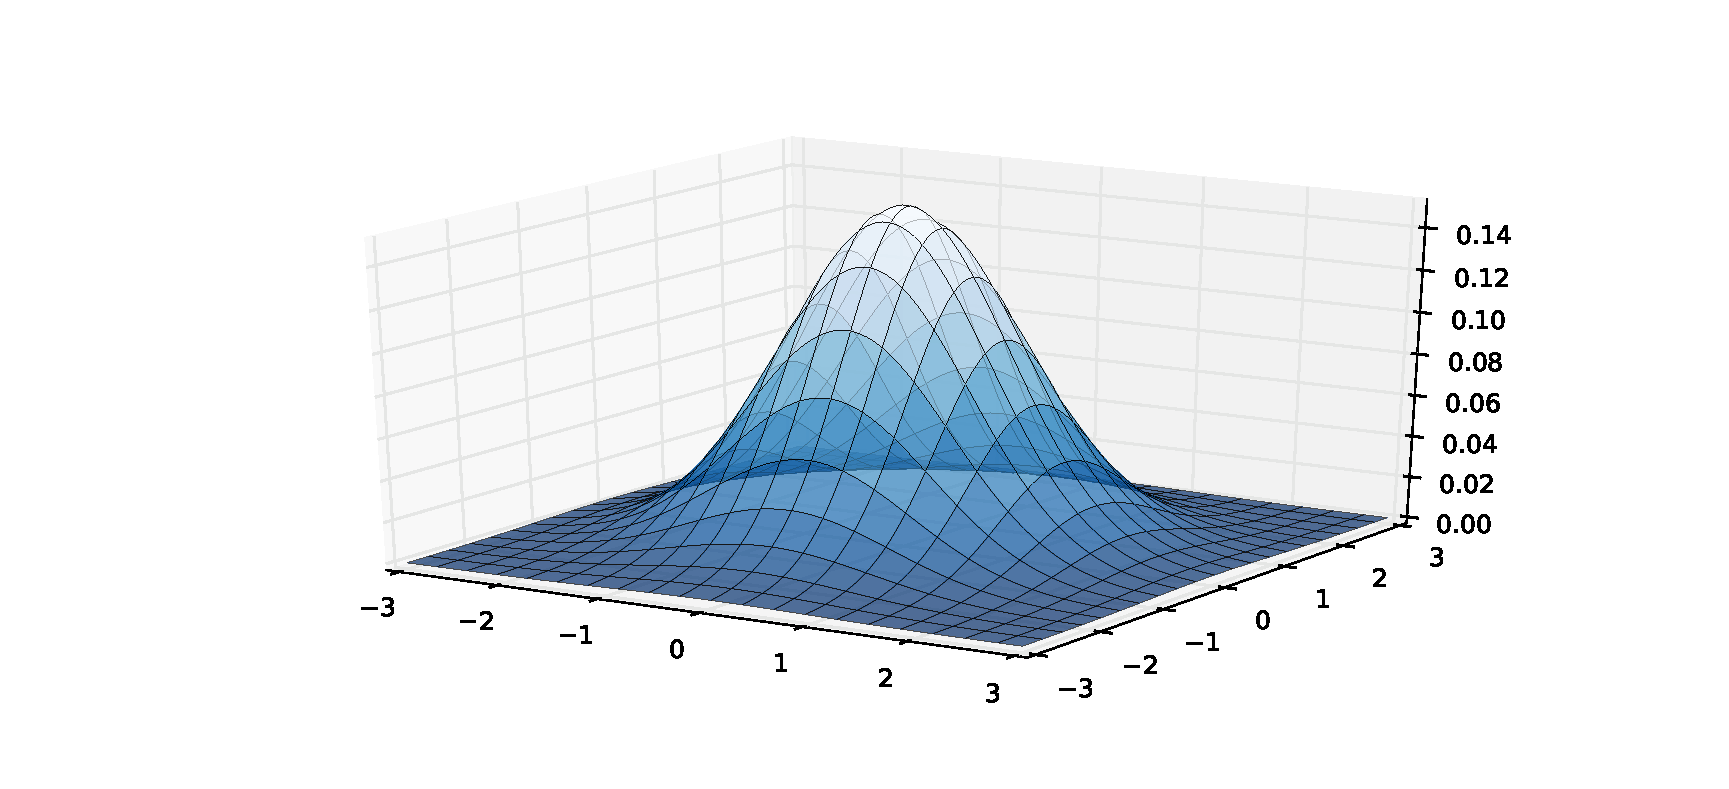
\includegraphics[trim={5em 5em 5em 5em}, clip]{bivar_gaussian_3d.pdf}}
   \caption{\label{f:bivar_gaussian_3d} Функция плотности двумерного стандартного нормального распределения}
   
    \end{figure}
    
\end{frame}
    
\begin{frame}
    
     \vspace{2em}
    \navy{Распределение произведения} $P_1, \ldots,
    P_N$ определяется следующим фактом:
    
     \vspace{1em}
    \Fact\eqref{ET-fa:prodist}
    Возьмем распределения $P_1, \ldots, P_N$ в $\RR$, существует единственное
    и определенное распределение $\mathring{P}$ в $\RR^N$, такое что
    %
    \begin{multline*}
        \mathring{P}(B_1 \times \cdots \times B_N)
        \\ = \prod_{n=1}^N P_n(B_n)
        \qquad \text{для всех } B_n \in \bB(\RR), \; n=1,\ldots, N       
    \end{multline*}
    
    \vspace{1em}
    Единственное, потому что распределения однозначно закреплены цилиндрическими 
    множествами $\mathbb{R}^{N}$ (смотрите страницу 128 в ET)
    
\end{frame}

\begin{frame}
    
    \vspace{2em}
    Возьмем любое распределение $P$ в $\RR^N$, $n$-ое \navy{частное
    распределение} $P$ --- это распределение в $\RR$ определенное как 
    %
    \begin{equation*}
        P_n(B)
        = P (\RR \times \cdots \times \RR \times B \times \RR \times \cdots
        \times \RR)
    \end{equation*}
    
    \vspace{.7em}
    Здесь $B$ --- $n$-ый элемент Декартого произведения
    
    \vspace{.7em}
    Эквивалентно, 
    %
    \begin{equation*}
    P_n(B) 
    = P \setntn{\bolds \in \RR^N}{\bolds^\T \bolde_n \in B}
    \end{equation*}
    
\end{frame}

\begin{frame}

    \vspace{2em}
    Из $P_n$ мы можем также получить \navy{частную функцию распределения $F_n$} с помощью 
    %
    \begin{equation*}
        \label{eq:ntf}
        F_{n}(s) := P_{n}( (-\infty, s] )
        \qquad (s \in \RR)
    \end{equation*}
    %
    (смотрите страницу~\pageref{ET-eq:ntf} в ET)
    
    \vspace{1em}
    Если $P_n$ абсолютно непрерывная, она имеет функцию плотности $p_n$
    
    Если совместное распределение $P$ имеет функцию плотности $p$, частное распределение 
    $P_n$ имеет функцию плотности $p_n$ -- ''интегрировать по другим переменным''
    
    \vspace{.7em}
    Например, двумерный случай:
    %
    \begin{equation*}
        p_1(s_1)
        = \int_{-\infty}^{\infty} p(s_1, s_2) \diff s_2
    \end{equation*}
    
\end{frame}

\begin{frame}
    
    \vspace{2em}
    \begin{figure}
       \begin{center}
        \scalebox{.44}{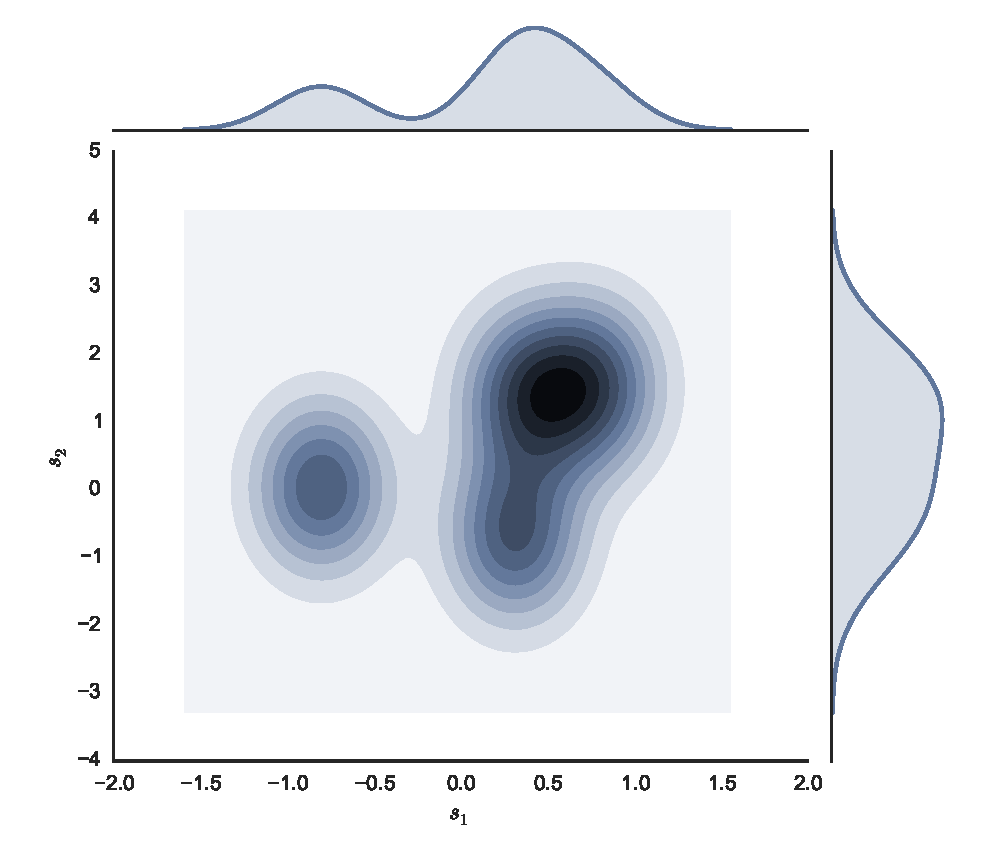
\includegraphics{jointplot.pdf}}
        \caption{\label{f:jointplot} Двумерная совместная функция плотности и две ее частных вариации}
       \end{center}
    \end{figure}
    
\end{frame}

\begin{frame}

    \vspace{2em}
    Совместное распределение не может быть получино только из частных
    \begin{itemize}
        \item частные не говорят нам о своем взаимодействии
    \end{itemize} 
    
    \vspace{1em}
    Исключение составляют случаи отсутствия взаимодействия - случай произведения функций распределения 
    
\end{frame}

\begin{frame}\frametitle{Распределения случайных векторов}
    
    \vspace{2em}
    Пусть $\boldx$ --- случайный вектор в $\RR^N$
    
    \vspace{1em}
    \navy{Распределение} $\boldx$ является вероятностной мерой $P$ на $\bB(\RR^N)$ 
    определяемая как
    %
    \begin{equation*}
        \label{eq:dmnu}
        P(B) = \PP\{\boldx \in B\}
        \qquad (B \in \bB(\RR^N))
    \end{equation*}
    %
    $P$ здесь также называется \navy{совместным распределением}
    $x_1,\ldots, x_N$, и мы пишем $\lL(\boldx) = P$
    
\end{frame}
    
\begin{frame}
    
    \vspace{2em}
    Совместное распределение представлено многомерной функцией распределения 
    $F \colon \RR^N \to [0, 1]$:
    %
    $$F(s_1,\ldots,s_N) = \PP\{ x_1 \leq s_1, \ldots, x_N \leq s_N\}$$
    %
    или, в векторной форме
    %
    \begin{equation*}
        F(\bolds) = \PP\{\boldx \leq \bolds\}
        \qquad (\bolds \in \RR^N)
    \end{equation*}
    
\end{frame}

\begin{frame}

    \vspace{2em}
    Когда распределение $P$
    абсолютно непрерывно, существует неотрицательная функция $p$ в $\RR^N$, такая что
    %
    \begin{equation*}
        \label{eq:defjd00}
        \int_B p(\bolds) \diff  \bolds = \PP\{\boldx \in B\}
        \qquad (B \in \bB(\RR^N))
    \end{equation*}
    %
    функция $p$ --- \navy{совместная функция плотности} $\boldx$
    
    \vspace{1em}
    Для выполнения вышеизложенного достаточно, чтобы 
    \begin{equation*}
    \label{eq:defjd}
    \int_{-\infty}^{s_N} 
    \cdots
     \int_{-\infty}^{s_1} 
    p(t_1,\ldots,t_N) 
    \diff t_1 \cdots \diff t_N
    = F(s_1,\ldots,s_N) 
    \end{equation*}
    %
    для всех $s_n  \in \RR$, $n=1,\ldots, N$ 
    
\end{frame}


\begin{frame}

    \vspace{2em}
    Если $\boldx = (x_1,\ldots, x_N)$ --- случайный вектор в $\RR^N$, то каждый $x_n$
    --- случайная величина в $\RR$
    
    \vspace{1em}
    Пусть $P_n = \lL(x_n)$, тогда: 
    %
    \begin{equation*}
        \label{eq:deffx2}
        P_n(B) = \PP \{x_n \in B \}
        \qquad (B \in \bB(\RR), \; n = 1, \ldots, N)
    \end{equation*}
    %

    $P_n$ называется \navy{частным распределением $x_n$}
    
    Если $P_1 = P_2 = \cdots = P_N$, то $x_1, \ldots, x_N$ \navy{одинаково распределены}
    
\end{frame}

\begin{frame}\frametitle{Нормальные случайные векторы}
    
    \vspace{2em}
    Случайная переменная $x$ 
    \navy{нормально распределена}, если $x = \mu + \sigma z$ для некоторых $\sigma \geq 0$
    
    Мы пишем $\lL(x) = \nN(\mu, \sigma)$
    
\end{frame}

\begin{frame}
    
    \vspace{2em}
    Случайный вектор $\boldx$ в $\RR^N$ \navy{многомерный нормальный}, если
    %
    \begin{equation*}
        \label{eq:imn}
        \boldx = \boldmu + \boldC \boldz
    \end{equation*}
    %
    где $\boldz$ --- стандартный нормальный случайный вектор размера $K \times 1$, 
    матрица $\boldC$ имеет размер $N \times K$ и вектор $\boldmu$ имеет размер $N \times 1$
    
    \vspace{1em}
    Если $\boldx$ многомерный нормальный, то мы пишем $\lL(\boldx ) =
    \nN(\boldmu, \boldSigma)$, где
    %
    \begin{equation*}
        \boldmu := \EE \boldx 
        \quad \text{и} \quad
        \boldSigma := \var \boldx
    \end{equation*}
    %
    Имеется $\boldSigma = \boldC\boldC^\T$ (вспомним факт 5.1.2 в ET)
    
\end{frame}

\begin{frame}
    
    \vspace{2em}
   $\lL(\boldx) = \nN(\boldmu, \boldSigma)$ не подразумевает, что
    $\boldx$ имеет многомерную нормальную функцию плотности
    \begin{itemize}
        \item распределение $\boldx$ может и не быть абсолютно непрерывным, 
        например если $\boldC = \boldzero$ 
    \end{itemize}
    
    \vspace{1em}
    Абсолютная непрерывность распределения $\boldx$ совпадает с 
    условиями, где $\boldSigma := \var \boldx$ несингулярна -- 
    несингулярность $\boldSigma$ будет верна тогда и только тогда, когда
    $\boldC^\T$ имеет полный ранг столбцов
    
\end{frame}

\begin{frame}
    
    \vspace{2em}
    \Fact\eqref{ET-fa:nipre}
    Пусть $\boldx$ --- случайный вектор в $\RR^N$. Следующие утверждения верны:
    %
    \begin{enumerate}
        \item вектор $\boldx$ многомерный нормальный тогда и только тогда, когда
            $\bolda^\T \boldx$ нормально распределено в $\RR$ для каждого
            постоянного вектора $\bolda$ размера $N \times 1$ 
        \item Если $\lL(\boldx) = \nN(\boldmu, \boldSigma)$, то 
            %
            \begin{equation*}
                  \lL(\boldA \boldx + \boldb) = \nN(\boldA \boldmu + \boldb, \boldA
                    \boldSigma \boldA^\T)  
            \end{equation*}
            %
            для всех постоянных согласованных $\boldA, \boldb$
    \end{enumerate}
    
\end{frame}

\begin{frame}

    \vspace{2em}
    Следствие: если $\boldx = (x_1,
    \ldots, x_N)$ многомерный нормальный, то частное распределение 
    $x_n$ одномерное нормальное
    
    Всегда ли совместное распределение $N$ одномерных нормальных случайных величин 
    является многомерным нормальным? 
    \begin{itemize}
        \item Ответ: нет
    \end{itemize}
    
\end{frame}

\begin{frame}\frametitle{Ожидания из распределений}

    \vspace{2em}
    Пусть $h \colon \RR^N \to \RR$ --- любая $\bB$-измеримая функция и
    $P$ --- распределение в $\RR^N$
    
    Функция $h$ теперь рассматривается как a случайная переменная в 
    $(\RR^N, \bB(\RR^N), P)$
    
    Математическое ожидание $h$ может быть записано как
    %
    \begin{equation}
        \label{eq:eph}
        \EEP h :=: \int h(\bolds) P(\diff \bolds)
    \end{equation}
    
\end{frame}

\begin{frame}

    \vspace{2em}
    \Fact\eqref{ET-fa:haspvec}
        Пусть $h \colon \RR^N \to \RR$ $\bB$-измерима и $P$ ---
        распределение в $\RR^N$. Если $P$ дискретное, с вероятностной функцией $\{p_j\}_{j
        \geq 1}$ и носителем распределения $\{\bolds_j\}_{j \geq 1}$, то
        %
        \begin{equation}
            \label{eq:hasp2}
            \int h(\bolds) P(\diff \bolds) = \sum_{j\geq 1} h(\bolds_j) p_j 
        \end{equation}
        %
        Если $P$ абсолютно непрерывное с функцией плотности $p$, то
        %
        \begin{equation}
            \label{eq:hasd2}
            \int h(\bolds)P(\diff \bolds) 
            = \int h(\bolds) p(\bolds) \diff \bolds
    \end{equation}
    
    правую сторону \eqref{eq:hasd2} следует понимать как 
    %
    \begin{equation*}
        \int_{-\infty}^\infty
            \cdots
            \int_{-\infty}^\infty
            h(s_1, \ldots, s_N) \,
            p(s_1,\ldots,s_N)  \,
            \diff s_1 \cdots \diff s_N
    \end{equation*}
    %
\end{frame}

\begin{frame}
    
    \vspace{2em}
    Как и в одномерном случае, такие объекты, как моменты, являются свойствами распределения

    \vspace{1em}
    Например, пусть $\boldx$ --- случайный вектор в $\RR^K$
    с $\lL(\boldx) = P$
    
    Ковариационная матрица $\var [\boldx]$ имеет $i,j$-ый элемент равный 
    $\EE [x_i x_j] - \EE[x_i]\EE[x_j]$
    
    Мы можем записать $\var [\boldx]$ относительно $P$. Если
    %
    \begin{equation*}
        \label{eq:vcd2}
        \boldSigma_P = (\sigma_{ij}) 
        \quad \text{, где} \quad
        \sigma_{ij} := \int (s_i s_j) P(\diff \bolds) 
            - \int s_i P(\diff \bolds) \cdot \int s_j P(\diff \bolds)
    \end{equation*}
    %
    тогда $\boldSigma_P = \var[\boldx]$
    
\end{frame}

\begin{frame}\frametitle{Независимость случайных величин}

    \vspace{2em}
    Множество $N$ случайных величин $x_1, \ldots, x_N$ \navy{независимо}, если
    %
    \begin{equation}
        \label{eq:bcap}
        \PP \bigcap_{n=1}^N \{x_n \in B_n\}
        = \prod_{n=1}^N \PP\{x_n \in B_n\} 
    \end{equation}
    %
    для любых $B_1, \ldots, B_N$, где каждый $B_n$ --- Борелевское подмножество $\RR$
    
    \vspace{1em}
    Случайные величины $x_1, \ldots, x_N$ независимы, когда множества вида 
    $\{x_1 \in B_1\}, \ldots, \{x_N
    \in B_N\}$ являются независимыми событиями
    
    Бесконечное множество случайных величин $\{x_n\}_{n=1}^{\infty}$ 
    независимо, если любое конечное подмножество  $\{x_n\}_{n=1}^{\infty}$ независимо
    
\end{frame}

\begin{frame}

    \vspace{2em}
    Эквивалентное определение независимости с использованием распределений
    
    Пусть $P$ --- совместное распределение $\boldx = (x_1, \ldots, x_N)$ и $P_n$ ---  
    его $n$-ое частное
    
    Так как
    $\cap_{n=1}^N \{x_n \in B_n\}
    = \{ (x_1, \ldots, x_N) \in B_1 \times \cdots \times B_N \}$, случайные
    величины $x_1, \ldots, x_N$ независимы, если
    %
    \begin{equation*}
        P(B_1 \times \cdots \times B_N) 
        = \prod_{n=1}^N P_n(B_n)
    \end{equation*}
    
    Элементы случайного вектора 
    независимы тогда и только тогда, когда их совместное распределение равняется 
    произведению их частных распределений 
    
\end{frame}

\begin{frame}

    \vspace{2em}
   Необходимое и достаточное условие независимости $x_1, \ldots, x_N$:
    %
    \begin{equation*}
        \label{eq:pdind}
        F(s_1,\ldots,s_N) 
        = \prod_{n=1}^N F_n(s_n)
    \end{equation*}
    %
    для всех $(s_1, \ldots, s_N) \in \RR^N$, где $F$ функция распределения $\boldx$ и
    $F_1, \ldots, F_N$ частные функциии распределения (почему?)
    
\end{frame}

\begin{frame}
    
    \vspace{2em}
    Если  распределение $\boldx$ абсолютно непрерывное, мы можем также проверить
    независимость с помощью его функции плотности: 
    
    \vspace{1em}
    \Fact\eqref{ET-fa:immd}
        Если $\boldx = (x_1, \ldots, x_N)$ имеет совместную функцию плотности $p$ и частные
        $p_1, \ldots, p_N$, то $x_1, \ldots, x_N$ независимы тогда и только тогда, когда
        %
        \begin{equation*}
            p (s_1,\ldots, s_N) = \prod_{n=1}^N p_n(s_n)
            \qquad \text{для всех} \quad
            (s_1, \ldots, s_N) \in \RR^N
        \end{equation*}
        
\end{frame}

\begin{frame}

    \vspace{2em}
    \Eg 
    
    Пусть $\lL(\boldx) = \lL(x_1, \ldots, x_N) = N(\boldmu, \boldSigma)$ 
    
    Предположим также, что 
    $\boldSigma$ диагональна, с $n$-ым диагональным элементом
    $\sigma_n > 0$, тогда $x_1, \ldots, x_N$ независимые
    
    Чтобы убедиться в этом, проверим для любых
    $\bolds = (s_1, \ldots, s_N) \in \RR^N$, имеется
    %
    \begin{align*}
        p(\bolds) 
        & = (2 \pi)^{-N/2} \determinant (\boldSigma)^{-1/2} 
        \exp \left\{ 
            - \frac{1}{2} (\bolds - \boldmu)^\T \boldSigma^{-1} (\bolds - \boldmu) 
        \right\}
        \\
        & = \frac{1}{(2 \pi)^{N/2} \prod_{n=1}^N \sigma_n}
        \exp \left\{ 
            - \frac{1}{2} \sum_{n=1}^N (s_n - \mu_n)^2 \sigma_n^{-2}
        \right\}
    \end{align*}
    
\end{frame}

\begin{frame}

    \vspace{2em}
    \Eg (прод.)
    Вычисление определителя и обратной матрицы $\boldSigma$ с 
    помощью фактов~\ref{ET-fa:dtmat} и \ref{ET-fa:powdm}
    
    Последнее выражение можно разложить дальше
    %
    \begin{equation*}
        p(\bolds) 
        =
        \prod_{n=1}^N \frac{1}{(2 \pi)^{1/2} \sigma_n}
            \exp \left\{ 
                \frac{-(s_n - \mu_n)^2}{2 \sigma_n^2}
            \right\}
         =
        \prod_{n=1}^N p_n(s_n)
    \end{equation*}
    %
    где $p_n$ --- функция плотности $\nN(\mu_n, \sigma^2_n)$

\end{frame}

\begin{frame}

    \vspace{2em}
    \Fact\eqref{ET-fa:imme}
   Если $x_1, \ldots, x_N$ независимые и каждый $x_n$ интегрируемый, то
   %
   \begin{equation*}
       \EE \left[ \prod_{n=1}^N x_n \right]
       = \prod_{n=1}^N \EE[ x_n ]
   \end{equation*}
   %
\end{frame}

\begin{frame}\frametitle{Независимость случайных векторов}

    \vspace{2em}
    Случайные векторы $\boldx_1, \ldots, \boldx_N$ in $\RR^K$ are called
    \navy{независимы}, если
    %
    \begin{equation*}
        \label{eq:bcapv}
        \PP \bigcap_{n=1}^N \{\boldx_n \in B_n\}
        = \prod_{n=1}^N \PP\{\boldx_n \in B_n\} 
    \end{equation*}
    %
    для любых $B_1, \ldots, B_N$, где каждый $B_n$ --- Борелевское подмножество $\RR^K$
    
\end{frame}

\begin{frame}
    
    \vspace{2em}
    \Fact\eqref{ET-fa:rviifi}
    Если $\boldx_1, \ldots, \boldx_N$ --- независимые случайные векторы в $\RR^K$ и 
    $f_1, \ldots, f_N$ --- любые $\bB$-измеримые функции,
    то $f_1(\boldx_1), \ldots, f_N(\boldx_N)$ также независимы.
    
    \Prf 
    Заметим, что $f_n(\boldx_n) \in B_n$ тогда и только тогда, когда $\boldx_n \in
    f^{-1}(B_n)$. Это ведет к
    %
    \begin{equation*}
        \bigcap_{n=1}^N \{f_n(\boldx_n) \in B_n\}
        = \bigcap_{n=1}^N \{\boldx_n \in f^{-1}(B_n)\}
    \end{equation*}
    %
    Применяем независимость $\boldx_1, \ldots, \boldx_N$
    %
    \begin{multline*}
        \PP
        \bigcap_{n=1}^N \{f_n(\boldx_n) \in B_n\}
        \\ = \prod_{n=1}^N \PP \{\boldx_n \in f^{-1}(B_n)\}
        = \prod_{n=1}^N \PP \{f_n(\boldx_n) \in B_n\}
    \end{multline*}
    %
    
\end{frame}

\begin{frame}

    \vspace{2em}
    \Fact\eqref{ET-fa:indzcov}
    Если $\boldx$ и $\boldy$ независимые, то $\cov(\boldx,\boldy) = 0$.
        
    Обратное не верно: можно найти примеры зависимых векторов с нулевой ковариацией.  
    Однако,

    \Fact\eqref{ET-fa:ucimin}
    Если $\boldx$ многомерно нормально распределен и $\boldA$ и $\boldB$ 
    согласованные постоянные матрицы, то $\boldA \boldx$ и
    $\boldB \boldx$ независимые тогда и только тогда, когда $\cov(\boldA \boldx, \boldB\boldx) = \boldzero$
        
\end{frame}

\begin{frame}

    \vspace{2em}
    \Fact\eqref{ET-fa:poci}
    Пусть $S$ --- любое линейное подпространство $\RR^N$, $\boldP := \proj S$ и
    $\boldM$ --- остаточная проекция. Если $\lL(\boldz) = \nN(\boldzero,
    \sigma^2 \boldI)$ в $\RR^N$ для некоторых $\sigma^2 > 0$, то $\boldP \boldz$ и
    $\boldM \boldz$ независимые
    
    \vspace{1em}
    \Fact\eqref{ET-fa:lcinorm}
        Если $w_1, \ldots, w_N$ независимые с $\lL(w_n) = \nN(\mu_n,
        \sigma_n^2)$ для всех $n$, то
        %
        \begin{equation*}
            \lL \left[ \alpha_0 + \sum_{n=1}^N \alpha_n w_n \right]
            = \nN \left( 
                \alpha_0 + \sum_{n=1}^N \alpha_n \mu_n,\;
                \sum_{n=1}^N \alpha_n^2 \sigma_n^2
                \right)
        \end{equation*}
        %
\end{frame}

\begin{frame}

    \vspace{1em}
    Суммы произвольных нормальных не всегда нормальны --- нам требуется 
    многомерное нормальное распределение
    
    \vspace{1em}
    В факте \eqref{ET-fa:lcinorm} выше:
    %
    $$\lL(w_1, \ldots, w_N) = \nN(\boldmu,
    \boldSigma)$$ 
    %
    где $\bolde_n^\T \, \boldmu = \mu_n$, и
    %
    $$\boldSigma =
    \diag(\sigma_1^2, \ldots, \sigma_N^2)$$
 
    
\end{frame}

\section{Copulas}

\begin{frame}

    \vspace{2em}
    \navy{Копула} $C$ в $\RR^N$ --- многомерная функция распределения определённая на
    единичном гиперкубе $[0, 1]^N$, такая что
    каждое ее частное распределение равномерно на $[0, 1]$
    
    $C$ --- функция вида
    %
    \begin{equation}
        \label{eq:icif}
        C(s_1, \ldots, s_N) = \PP \{u_1 \leq s_1, \ldots, u_N \leq s_N\}
    \end{equation}
    %
    Где $0 \leq s_n \leq 1$ и $\lL(u_n) = U[0, 1]$ для всех $n$
    
    \vspace{1em}
    Пока каждый $u_n$ имеет фиксированное частное распределение, существует 
    бесконечно много способов составить совместное распределение
        
\end{frame}

\begin{frame}

    \vspace{2em}
    \Eg Функция $C(s_1, s_2) = s_1 s_2$ on $[0, 1]^2$ называется
    \navy{независимая копула}
    
    \vspace{1em}
    Частные распределения $C(s_1, 1) =
    s_1$ и $C(1, s_2) = s_2$ как и требуется
    
    (Это функции распределения для
    $U[0, 1]$ распределения)

\end{frame}

\begin{frame}

    \vspace{2em}
    \Eg
    \navy{Копула Гумбеля} --- класс функций в $[0, 1]^2$, определяемый как
    %
    \begin{equation*}
        C(s_1, s_2) = 
        \exp 
        \left\{
            - \left[ 
                (-\ln s_1)^\theta + (-\ln s_2)^\theta
            \right]^{1/\theta}
        \right\}
        , \quad (\theta \geq 1)
    \end{equation*}
    %
    \navy{Копула Клейтона} определяется как
    %
    \begin{equation*}
        C(s_1, s_2) = 
        \left\{
            \max \left[
                s_1^{-\theta} +  s_2^{-\theta} -1, \, 0
                \right]
        \right\}^{-1/\theta}
        ,\quad (\theta \geq -1, \, \theta \not= 0)
    \end{equation*}
   
    Обе они принадлежат к общему классу, называемому \navy{Архимедовы копулы}

\end{frame}

\begin{frame}

    \vspace{2em}
    Мы можем взять равномерные функции распределения
    $F_1, \ldots, F_N$ и копулу $C$, чтобы создать многомерную функцию распределения в
    $\RR^N$ с помощью
    %
    \begin{multline}
        \label{eq:ffcop}
        F(s_1, \ldots, s_N) = C(F_1(s_1), \ldots, F_N(s_N))
        \\ (s_n \in \RR, \, n=1, \ldots, N)
    \end{multline}
    
    \vspace{1em}
    Польза: разделяем определение частных и определение совместного распределения
    
\end{frame}

\begin{frame}

    \vspace{2em}
    \Eg
    \cite{bonhomme2009assessing} использует копулы для моделирования одного компонента динамики заработка в исследовании, основанном на трехлетних панельных данных (French Labor Force Survey)
    
    Разделы относительно большие (около 30 000), что позволяет гибко моделировать частные распределения с помощью смеси нормальных
    
    Однако, размер временного ряда короткий, поэтому используется семейство копул с одним параметром для привязки частных во времени не трудозатратным способом

\end{frame}

\begin{frame}

    \vspace{2em}
    \Thm\eqref{ET-t:sklar}
        Если $F$ --- некоторая функция распределения в $\RR^N$ с частными $F_1, \ldots, F_N$,
        то существует копула $C$, такая что \eqref{eq:ffcop} выполняется. Если каждый
        $F_n$ непрерывен, то это представление является единственным.
        
\end{frame}

\begin{frame}

    \vspace{2em}
    Если $F_1, \ldots, F_N$ равномерные нормальные, то $C(F_1(s_1), \ldots, F_N(s_N))$
    будут равняться многомерной нормальной функции распределения для одного варианта копулы,
    называемой Гауссовой копулой
    
    \vspace{2em}
    Другие варианты приводят к другим распределениям
    
\end{frame}

\begin{frame}
    
    \vspace{2em}
    \begin{figure}
       \centering
       \scalebox{.44}{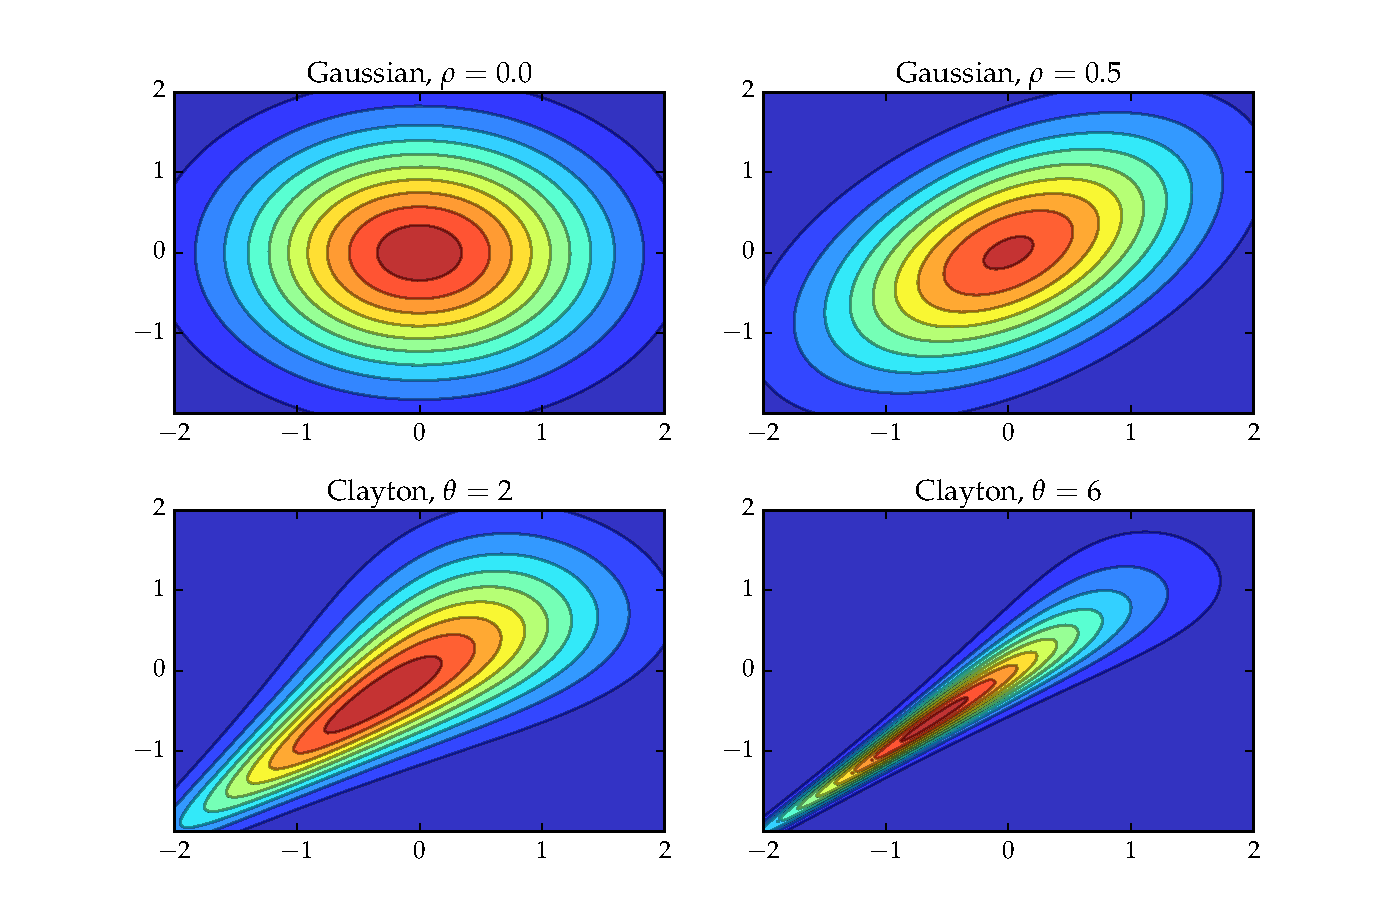
\includegraphics[trim={0 2em 0 2em}, clip]{copula.pdf}}
       \caption{\label{f:copula} Двумерный Гауссовская (вверху) и не-Гауссовская (внизу)}
    \end{figure}
    
\end{frame}

	\section{Свойства именных распределений}

\begin{frame}\frametitle{Свойства именных распределений}

    \vspace{2em}
    \Fact
    \eqref{ET-fa:schis}
    Если $x_1,\ldots,x_N$ независимые и $\lL(x_n) = \chi^2(k_n)$,
     то $\lL(\sum_n x_n) = \chi^2(\sum_n k_n)$
    
    \vspace{2em}
    \Fact
    \eqref{ET-fa:astudt}
    Если $z$ и $x$ независимые с $\lL(z) = \nN(0,1)$ и $\lL(x) = \chi^2(k)$, 
    то 
    %
    \begin{equation*}
        z \sqrt{\frac{k}{x} } 
        \;\;
        \text{ распределено как $t$ с $k$ степенями свободы}
    \end{equation*}
    

\end{frame}

\begin{frame}

    \vspace{2em}
    \Fact
    \eqref{ET-fa:ssnac}
    Если $\lL(z_1, \ldots, z_N) = \nN(\boldzero, \boldI)$, то
    $\lL(\sum_{n=1}^N z_n^2) = \chi^2(N)$. 
    
    \vspace{2em}
    \Fact
    \eqref{ET-fa:mcfi}
    Если $\lL(\boldz) = \nN(\boldzero, \boldI)$ и $\boldA$ симметрична и
    идемпотентна, то 
    %
    \begin{equation*}
        \lL \left( \boldz^\T \boldA \boldz \right) = \chi^2(K)  
        \quad \text{, где} \quad
        K := \trace \boldA
    \end{equation*}
    
    \vspace{1em}
    Упражнение: получите факт \eqref{ET-fa:mcfi} из факта \eqref{ET-fa:ssnac}.
    (Смотрите страницу~\pageref{ET-fa:mcfi} в ET)
    
\end{frame}

\section{Условия и ожидание}

\begin{frame}\frametitle{Условия и ожидание}

    \vspace{2em}
    Условное ожидание --- одно из важнейших понятий как в экономической теории, 
    так и в эконометрике
    
    В этом разделе дается построение математического ожидания, основанное на проекции:
    
    \begin{itemize}
        \item условное математическое ожидание как оптимальное предсказание 
        с учетом ограниченной информации
    \end{itemize}

\end{frame}

\begin{frame}\frametitle{Условные функции плотности}

    \vspace{2em}
    Сначала обсуждение условных функций плотности 
    
    Пусть $x_1$ и $x_2$ --- случайные величины. \navy{Условиная функция плотности} 
    $x_2$ при заданном $x_1 = s_1$ определяется как 
    %
    \begin{equation*}
        p(s_2 \given s_1) 
            := \frac{p(s_1, s_2)}{p(s_2)}
    \end{equation*}
    
    Здесь $p$ может обозначать совместную, частную или условную функцию плотности, 
    определяемую аргументом
    
\end{frame}

\begin{frame}

    \vspace{2em}
    Закон полной вероятности расширяется до случая с функциями плотности
    следующим образом: Если $(x_1, x_2)$ --- случайный вектор в $\RR^2$, то
    %
    \begin{equation*}
        \label{eq:dltp}
        p(s_2)
        = \int_{-\infty}^{\infty} p(s_2 \given s_1) p(s_1) \diff s_1
        \qquad \qquad 
        (s_2 \in \RR)
    \end{equation*}
    
    \Prf 
    Зафиксируем $s_2 \in \RR$ и проинтегрируем совместную функцию плотности, чтобы получить частную, получается
    %
    $$
        p(s_2) = \int_{-\infty}^{\infty} p(s_1, s_2) \diff s_1
    $$
    Сочетаем с $p(s_2 \given s_1) = p(s_1, s_2)/p(s_1)$, чтобы получить результат
    
\end{frame}

\begin{frame}

    \vspace{2em}
    Закон Байеса также расширяется до случая с функциями плотности:
    %
    \begin{equation*}
        \label{eq:brdc}
        p(s_2 \given s_1) = \frac{p(s_1 \given s_2) p(s_2)}{p(s_1)}
    \end{equation*}

\end{frame}

\begin{frame}

    \vspace{2em}
    Условная функция плотности $x_{k+1},\ldots, x_N$ при $x_1 = s_1,\ldots, x_k =
    s_k$ определяется как
    %
    \begin{equation*}
        \label{eq:condden}
        p(s_{k+1},\ldots,s_N \given s_1,\ldots,s_k) 
            = \frac{p(s_1,\ldots,s_N)}{p(s_1,\ldots,s_k)}
    \end{equation*}
    
    \vspace{1em}
    Перегруппируйте, чтобы получить полезное разложение совместной функции плотности:
    %
    \begin{equation*}
        \label{eq:decompjd}
        p(s_1,\ldots,s_N) 
        = p(s_{k+1},\ldots,s_N \given s_1,\ldots,s_k) p(s_1,\ldots,s_k)
    \end{equation*}
    
\end{frame}

\begin{frame}

    \vspace{2em}
    Предположим, мы хотим предсказать случайную переменную $y$ с помощью другой переменной $x$
    
    Возьмем $x$ такой, что $x$ и $y$, как ожидается, будут близки при большинстве реализаций неопределенности
    
    \vspace{1em}
    Но что значит ''ожидаются близкими''?
    
\end{frame}

\begin{frame}

    \vspace{2em}
    \navy{Среднеквадратическая ошибка} (MSE)
    $$\EE [ (x -
    y)^2 ]$$
    
    \navy{Среднеквадратическое отклонение}:
    %
    \begin{equation}
        \label{eq:ndrv}
        \| x - y \| := \sqrt{ \EE [ (x - y)^2 ] }
    \end{equation}
     
    Есть много параллелей между обычным векторным пространством с эвклидовой нормой и 
    множеством случайных величин в сочетании с ''нормой'', определенной в \eqref{eq:ndrv} 
    --- мы формализуем эти идеи далее
    
\end{frame}

\begin{frame}

    \vspace{2em}
    Первым геометрическим понятием, которое мы определили для векторов, было скалярное произведение
    
    Аналогично, определим \navy{скалярное произведение между двумя случайными величинами} $x$ и $y$
    %
    \begin{equation*}
        \label{eq:ipl2}
        \inner{x, y} := \EE[xy]
    \end{equation*}
    
    \vspace{1em}
    Неравенство Коши — Буняковского для случайных величин говорит нам, что
    $\EE[xy]$ должен быть конечным и определенным всюду, 
    где $x$ и $y$ оба имеют конечные вторые моменты
    
\end{frame}

\begin{frame}
    
    \vspace{2em}
    Множество случайных величин с конечными вторыми моментами обычно обозначается как $L_2$ 
    %
    \begin{equation*}
        L_2 
        := \{ \text{ все случайные величины } x \text{ в } (\Omega, \fF, \PP)
        \text{ с } \EE [x^2] < \infty \}
    \end{equation*}

    \Fact\eqref{ET-fa:innpp2}
    Для любых $\alpha, \beta \in \RR$ и любых $x, y, z \in L_2$ следующие утверждения верны:
    %
    \begin{enumerate}
        \item $\inner{x, y} = \inner{y, x}$.
        \item $\inner{\alpha x, \beta y} =  \alpha \beta \inner{x, y}$.
        \item $\inner{x, \alpha y + \beta z} =  \alpha
            \inner{x, y} + \beta \inner{x, z}$.
    \end{enumerate}
    %
    Свойства следуют из определения скалярного произведения и линейности $\EE$
    
    Сравните приведенное выше с фактом~\ref{ET-fa:innpp} в ET для векторов в эвклидовом пространстве
    
\end{frame}

\begin{frame}

    \vspace{2em}
    Определим \navy{$L_2$ норму} как
    %
    \begin{equation*}
        \label{eq:rvnorm}
        \| x \| 
        := \sqrt{ \inner{x, x} } 
        := \sqrt{ \EE[x^2] } 
        \qquad (x \in L_2)
    \end{equation*}
    
    Норма дает понятие расстояния $\|x - y\|$ между случайными
    величинами что согласуется с понятием среднеквадратического отклонения
    
    \vspace{1em}
    \Fact\eqref{ET-fa:l2se}
    Для любых $\alpha \in \RR$ и любых $x, y \in L_2$, следующие утверждения верные:
    %
    \begin{enumerate}
        \item $\| x \| \geq 0$ и $\| x \| = 0$ тогда и только тогда, когда
            $x = 0$
        \item $\| \alpha x \| = |\alpha| \| x \|$
        \item $\| x + y \| \leq  \| x \| + \| y \|$
        \item $| \! \inner{x, y}\!  | \leq  \| x \| \| y \|$
    \end{enumerate}
    
\end{frame}

\begin{frame}

    \vspace{2em}
    Свойство 2. приведенного выше факта является непосредственным из определения нормы и линейности $\EE$
    
    Свойство 3.
    называется \navy{неравенством треугольника}, как и в векторном случае
    
    Свойство 4. --- это просто \navy{неравенство Коши — Буняковского} для случайных величин со 
    страницы~\pageref{ET-fa:csrv}
    
    Как и в векторном случае, неравенство треугольника доказывается неравенством Коши - Буняковского (смотрите упражнение~\ref{ET-ex:csrv})
    
\end{frame}

\begin{frame}

    \vspace{2em}
    Относительно 1., $\| x \| = 0$ не подразумевает, что $x(\omega) = 0$ для всех $\omega \in \Omega$
    
   Мы можем сказать, что если $\| x \| = 0$, то $\PP\{x =0\} =1$
    
    \vspace{1em}
    При работе с $L_2$, принято соглашение не различать случайные величины, различающиеся с нулевой вероятностью.
    
\end{frame}

\begin{frame}\frametitle{Линейные подпространства в $L_2$}

    \vspace{2em}
    Любая \navy{линейная комбинация} случайных величин с конечной дисперсией
    
    \begin{equation}
        \alpha_1 x_1 + \cdots \alpha_K x_K,
        \qquad \alpha_k \in \RR, \; x_k \in L_2
    \end{equation}
    %
    снова в $L_2$
    
    Когда $X$ --- подпространство $L_2$, множество конечных линейных комбинаций,
    которое может быть сформировано из элементов $X$, называется \navy{линейной оболочкой}
    $X$, и оюозначается как $\Span X$
    
\end{frame}

\begin{frame}

    \vspace{2em}
    \Eg
    Если $x \in L_2$ и $\1 := \1_\Omega$ постоянная случайная переменная, 
    всегда равная $1$, то $\Span\{\1, x\}$ --- множество случайных величин
    %
    \begin{equation}
        \label{eq:llasp}
         \alpha + \beta x 
         := \alpha \1 + \beta x
         \quad \text{для скаляров} \quad
         \alpha, \beta   
    \end{equation}
    %
    Это множество $\lL$ введенное, когда мы
    обсуждали лучшие линейные предикторы
    
\end{frame}

\begin{frame}

    \vspace{2em}
    Подмножество $S$ множества $L_2$ называется 
    \navy{линейным подпространством} $L_2$, если оно замкнуто относительно 
    сложения и умножения на скаляр
    \begin{itemize}
        \item для каждого $x, y \in S$ и $\alpha, \beta \in \RR$,
    мы имеем $\alpha x + \beta y \in S$
    \end{itemize}

    \vspace{1em}
    \Eg
    Линейная оболочка любого множества элементов $L_2$ --- линейное подпространство в $L_2$

\end{frame}

\begin{frame}

    \vspace{2em}
    \Eg
    Множество $Z := \setntn{x \in L_2}{\EE x = 0}$ является 
    линейным подпространством $L_2$, так как 
    %
    \begin{equation*}
        x, y \in Z
        \text{ и }
        \alpha, \beta \in \RR
         \implies
        \EE[\alpha x + \beta y] = \alpha \EE[x] + \beta \EE[y] = 0
    \end{equation*}
    
    \vspace{1em}    
    Как и в $\RR^N$, \navy{ортонормированный бизис} линейного подпространства $S$ пространства $L_2$ 
    --- множество $\{u_1, \ldots, u_K\} \subset S$ со свойством
    %
    \begin{align*}
        \inner{u_j, u_k}  = \1\{j = k\}
       \\  \quad \text{и} \quad
        \Span\{u_1, \ldots, u_K\} = S
    \end{align*}

\end{frame}

\begin{frame}

    \vspace{2em}
    \Eg
    Пусть $x \in L_2$ такой, что $S := \Span\{\1, x\}$ множество случайных величин
    %
    \begin{equation}
         \alpha + \beta x 
         := \alpha \1 + \beta x
         \quad \text{for scalars} \quad
         \alpha, \beta   
    \end{equation}
    
    Если мы определим
    %
    \begin{equation*}
        u_1 := \1 
        \quad \text{и} \quad
        u_2 := \frac{x - \mu}{\sigma_x}  
    \end{equation*}
    %
    Тогда 
    %
    \begin{equation*}
        \inner{ u_1, u_2 } 
        = \EE[u_1 u_2] 
        = \EE \left[ \frac{x - \mu}{\sigma_x} \right]
        = 0
    \end{equation*}
    %
    Ясно, что $\|u_1\| = \|u_2\| = 1$, так что эта пара ортонормирована
    
    Также просто показать, что $\Span\{u_1, u_2\} =
    \Span\{\1, x\}$, значит $\{u_1, u_2\}$ ортонормированный базис для $S$
    
\end{frame}

\begin{frame}\frametitle{Проекции в $L_2$}

    \vspace{2em}
    Как и в евклидовом случае, если $\inner{x,y}=0$, мы говорим, что $x$ и $y$
    \navy{ортогональны}, и пишем \navy{$x \perp y$}
    
    \vspace{1em}
    \Fact
    Если $x, y \in L_2$ и $\EE x=0$ или $\EE y=0$, то $x \perp y
    \iff  \cov[x,y] = 0$
    
\end{frame}

\begin{frame}
    
    \vspace{2em}
    Возьмем $y \in L_2$ и
    линейное подпространство $S \subset L_2$, мы ищем ближайший элемент $\hat y$ множества $S$
    к $y$
    
    Близость по норме $L_2$, так что $\hat y$ решение минимизации
    $\| y - z \|$ для всех $z \in S$
    
    Мы ищем
    %
    \begin{equation}
        \label{eq:mproj2}
        \hat y 
        = \argmin_{z \in S} \|y - z\|
        = \argmin_{z \in S} \sqrt{\EE [ (y - z)^2 ]}
    \end{equation}
    %

\end{frame}

\begin{frame}

    \vspace{2em}
    Следующая теорема имитирует теорему об ортогональной проекции, которую мы уже видели:
    
    \vspace{.7em}
    \Thm\eqref{ET-t:opt4}
    Пусть $y \in L_2$ и $S$ --- любое непустое замкнутое
    линейное подпространство $L_2$
    
    Следующие утверждения верны:
    %
    \begin{enumerate}
        \item задача оптимизации \eqref{eq:mproj2} имеет ровно одно решение
        \item $\hat y \in L_2$ является единственным решением
    \end{enumerate}
    %
    Утверждение, что $S$ замкнуто значит, что $\{x_n \} \subset S$ и $x
    \in L_2$ с $\| x_n - x \| \to 0$ подразумевает $x \in S$ ---  условие истинное
    для всех линейных подпространств, с которыми мы хотим работать
    
\end{frame}

\begin{frame}

    \vspace{2em}
    Аналогично в случае $\RR^N$, случайная переменная $\hat y$ выше 
    называется \navy{ортогональной проекцией $y$ на $S$}
    
    Возьмем фиксированное $S$, операция
    %
    \begin{equation*}
        y \; \mapsto \text{ ортогональная проекция $y$ на } S
    \end{equation*}
    %
    --- функция из $L_2$ в $L_2$:

    \begin{itemize}
        \item функция называется \navy{ортогональной проекцией на $S$}
        \item функция обозначается как $\boldP$ 
        \item мы пишем $\boldP = \proj S$
    \end{itemize}
    
\end{frame}

\begin{frame}
    
    \vspace{2em}
    Для каждого $y \in L_2$, $\boldP y$ отображение $y$ с помощью
    $\boldP$, которое является ортогональной проекцией $\hat y$
    \begin{itemize}
        \item интерпретируем $\boldP y$ как \emph{лучший преликтор $y$ из 
        множества случайных величин, содержащегося в $S$}
    \end{itemize}
    
\end{frame}

\begin{frame}

    \vspace{2em}
    \Fact\eqref{ET-fa:l2opt}

    Если $S$ --- любое линейное подпространство $L_2$, и $\boldP = \proj S$, то
    %
    \begin{enumerate}
        \item $\boldP$ --- линейная функция.
    \end{enumerate}
    %
    Более того, для любых $y \in L_2$, получается
    %
    \begin{enumerate}
        \setcounter{enumi}{1}
        \item $\boldP y \in S$,
        \item $y - \boldP y \perp S$,
        \item $\| y \|^2 = \| \boldP y \|^2 + \| y - \boldP
            y \|^2$,
        \item $\| \boldP y \| \leq \| y \|$, и
        \item $\boldP y = y$ тогда и только тогда, когда $y \in S$.
    \end{enumerate}
    %
    В 1, $\boldP$ линейна значит, что $\boldP(\alpha x + \beta y) =
    \alpha \boldP x + \beta \boldP y$ для всех $x, y \in L_2$  и $\alpha,\beta
    \in \RR$
    
\end{frame}

\begin{frame}

    \vspace{2em}
    \Fact\eqref{ET-fa:subsubl2}
    Пусть $S_i$ --- линейное подпространство $L_2$ для $i=1,2$ и $\boldP_i =
    \proj S_i$. Если $S_1 \subset S_2$, то
        $\boldP_1 \boldP_2 y = \boldP_1 y$ для всех $y \in L_2$
        
    \vspace{1em}
    \Fact\eqref{ET-fa:l2opt2}
    Если $\{u_1, \ldots, u_K\}$ --- ортонормированный базис $S$, то для всех $y
    \in L_2$,
    %
    \begin{equation}
        \label{eq:projon2}
        \boldP y = \sum_{k=1}^K \inner{y, u_k} \, u_k
    \end{equation}
    
\end{frame}

\begin{frame}

    \vspace{2em}
    \Eg
    \eqref{ET-eg:projam}
    Среднее случайной переменной $x$ можно рассматривать как 
    'лучший предиктор $x$ среди множества констант''  
    
    Пусть $S := \Span\{\1\}$, где $\1 := \1_\Omega$,
    и $\boldP := \proj S$
    
    Объект $\boldP x$ как раз лучший предиктор
    $x$ в классе постоянных случайных величин
    
   Не удивительно, что $\boldP x = \mu \1$, где $\mu := \EE x$
    
    Самый простой способ проверить это --- заметить, что $\{\1\}$ является
    ортонормированным множеством, охватывающим $S$, и следовательно, по \eqref{eq:projon2},
    %
    \begin{equation*}
        \boldP x 
        = \inner{x, \1} \, \1
        = \EE[x \1] \1 = \EE[x] \1 = \mu \, \1
    \end{equation*}
    %
    Вы можете также проверить утверждение, что $\mu \1$ --- проекция $x$ на
    $S$, проверив условия в (ii) теоремы~\ref{ET-t:opt4}
    

\end{frame}

\begin{frame}

    \vspace{2em}
    \Eg
   
    Зафиксируем $x, y \in L_2$ и рассмотрим проецирование $y$ на $S := \Span\{\1,
    x\}$
    
    Множество $S$ является множеством случайных величин
    %
    \begin{equation*}
         \alpha + \beta x 
         := \alpha \1 + \beta x
         \quad \text{для скаляров} \quad
         \alpha, \beta   
    \end{equation*}
    
    Задача проецирования $y$ на $S$ is эквивалентна задаче поиска лучшего линейного предиктора
    из \S\ref{ET-ss:blp}
    
    Для реализации отзыва проекции 
    %
    \begin{equation*}
        u_1 := \1 
        \quad \text{и} \quad
        u_2 := \frac{x - \mu}{\sigma_x}  
    \end{equation*}
    %
    сформируем ортонормированный базис для $S$
    
\end{frame}
    
\begin{frame}

    \vspace{2em} 
    Пусть $\boldP = \proj S$, применим факт \eqref{ET-fa:l2opt2}, получаем
    %
    \begin{equation*}
        \boldP y 
         = \la y, u_1 \ra u_1 + \la y, u_2 \ra u_2
         = \EE[ y ] + 
            \frac{\cov[x, y]}{\var[x]}(x - \EE[x])
    \end{equation*}
    
    Альтернативно
    %
    \begin{equation*}
        \boldP y 
        = \alpha^* + \beta^* x
        \quad
    \end{equation*}
    
    \begin{equation*}
        \text{где} \quad
        \beta^* := \frac{\cov[x, y]}{\var[x]}
        \quad \text{и} \quad
        \alpha^* := \EE[y] - \beta^* \EE[x]
    \end{equation*}
    %
\end{frame}

\begin{frame}\frametitle{Регрессия населения}

    \vspace{2em}
    Рассмотрим расширение задачи поиска лучшего линейного предиктора, описанной выше, до задачи, в которой информация для прогнозирования $y$ --- случайный вектор $\boldx$ в $\RR^K$ 
    
    Мы ищем $L_2$ ортогональную проекцию $y$ на линейное подпространство:
    %
    \begin{equation*}
    \Span\{\boldx\} 
    := \text{ случайные величины вида
        $\boldx^\T \boldb$ для некоторых $\boldb \in \RR^K$} 
    \end{equation*}
    
    \vspace{1em}
    Предположим, что $\EE[ \boldx^\T \boldx] < \infty$
    

\end{frame}


\begin{frame}
    
    \vspace{2em}
    \Fact\eqref{ET-fa:mpr}
    Если $\EE[\boldx \boldx^\T]$ положительно определена, то проекция $\boldP y$ любого $y
    \in L_2$ на $\Span\{\boldx\}$ определяется как
    %
    \begin{equation*}
        \label{eq:mpr}
      \hat y = \boldx^\T \boldb^*      
      \quad \text{где} \quad
      \boldb^* := \EE[\boldx \boldx^\T]^{-1} \EE[\boldx y]
    \end{equation*}

    
    \vspace{1em}
    Упражнение~\ref{ET-ex:mpr} просит доказать вышеизложенный факт 
    
    Положительная определенность
    $\EE[\boldx \boldx^\T]$ обеспечивает обратимость, значит
    $\boldb^*$ однозначно определено
    
    По определению ортогональных проекций, $\boldb^*$ обязательно
    удовлетворяет
    %
    \begin{equation*}
        \boldb^* = \argmin_{\bolda \in \RR^K} \EE[ (y - \boldx^\T \bolda)^2 ]
    \end{equation*}
    %
\end{frame}

\begin{frame}

    \vspace{2em}
    Задача линейного прогнозирования рассматривается также под названием \navy{линейная регрессия 
    	населения}
    \begin{itemize}
        \item ''население'', потому что мы используем
            истинное совместное распределение $(\boldx, y)$, когда считаем ожидания
    \end{itemize}
    
    \vspace{1em}
    У регрессии популяции есть аналог, называемый многомерной линейной регрессией, основанный на наблюдениях $(\boldx, y)$ -- мы обсудим это в главе~\ref{ET-c:reg}
    
\end{frame}

\begin{frame}\frametitle{Измеримость}

    \vspace{2em}
    Мы не всегда хотим ограничиваться линейными прогнозами
    
    Чтобы отказаться от требования линейности, изменим линейное подпространство, используемое для 
    проецирования, из множества линейных функций $\boldx$ на множество произвольных функций
    $\boldx$
    
    В результате, лучший предиктор --- это условное математическое ожидание относительно $\boldx$

\end{frame}

\begin{frame}
    
    \vspace{2em}
    Подпространством произвольных действительных функций от
    $\boldx$ называются $\boldx$-измеримые функции

    Пусть $\gG := \{x_1, \ldots, x_D\}$ --- любое множество случайных величин
    и $z$ --- любая другая случайная величина
    
    Переменная $z$ \navy{$\gG$-измерима}, если
    существует $\bB$-измеримая функция $g \colon \RR^D \to \RR$, такая что
    %
    \begin{equation*}
        \label{eq:gmeas}
        z = g(x_1, \ldots, x_D)
    \end{equation*}
    %
    \begin{itemize}
        \item равенство между случайными величинами следует интерпретировать поточечно
    \end{itemize}
    
\end{frame}

\begin{frame}

    \vspace{2em}
    $\gG$ иногда упоминается как \navy{информационное множество}
    
    Мы также будем писать $\boldx = (x_1, \ldots, x_D)$ и говорить, что
    $z$ является $\boldx$-измеримым
    
    Аналогичная терминология будет использоваться для скаляров и матриц
    \begin{itemize}
        \item например, если $\boldX$ --- случайная матрица, то
        $\boldX$-измеримость означает $\gG$-измеримость, когда $\gG$ содержит все элементы $\boldX$
    \end{itemize}
    
    \vspace{1em}
    Интуиция: $\gG$-измеримость $z$ значит, что $z$ полностью определяется элементами в $\gG$
    
\end{frame}

\begin{frame}

    \vspace{2em}
    \Eg
    Пусть $x, y$ и $z$ --- случайные величины и пусть $\alpha$ и $\beta$ --- скаляры
    
    Если $z = \alpha x + \beta y$, то $z$
    $\{x, y\}$-измеримо (возьмем $g(s, t) := \alpha s + \beta t$)  

    \vspace{1em}
    \Eg
    Если $x_1, \ldots, x_N$ --- случайные величины
    и $\gG := \{x_1, \ldots, x_N\}$, то выборочное среднее $\bar x_N :=
    \frac{1}{N} \sum_{n=1}^N x_n$ является $\gG$-измеримым.
\end{frame}

\begin{frame}

    \vspace{2em}
    \Eg
    Пусть $\boldx$ и $y$ независимые и невырожденные
    
    Тогда $y$ не является $\boldx$-измеримым. Если бы он таким являлся, мы бы имели $y =
    g(\boldx)$ для некоторой функции $g$, противоречащее независимости $\boldx$ и $y$
    
    \vspace{1em}
    \Eg
    Пусть $y = \alpha$, гле $\alpha$ --- константа
    
    Эта вырожденная случайная величина является $\gG$-измеримой для любых информационных множеств $\gG$, потому что $y$ уже детерминированный
    
    Например, если $\gG = \{x_1, \ldots, x_p\}$, то
    мы можем взять $y = g(x_1, \ldots, x_p) = \alpha + \sum_{i=1}^p 0 x_i$  

\end{frame}

\begin{frame}

    \vspace{2em}
    \Fact\eqref{ET-fa:lcapom}
        Пусть $\alpha, \beta$ --- любые scalars, и пусть $x$ и $y$ --- случайные
        величины. Если $x$ и $y$ являются $\gG$-измеримыми, то $u := xy$ и
        $v := \alpha x + \beta y$ также являются $\gG$-измеримыми
    
    \vspace{1em}
    Предположим, что $\gG \subset L_2$ и рассмотрим множество
    %
    \begin{equation*}
        L_2(\gG) 
        := \{ \text{все $\gG$-измеримые случайные величины в } L_2 \}
    \end{equation*}
    
   
    С учетом факта~\ref{ET-fa:lcapom}:

    \Fact
        Для любых $\gG \subset L_2$, множество $L_2(\gG)$ --- линейное подпространство $L_2$
    
    Это дает нам подпространство для проецирования, что позволяет нам определять условные математические ожидания
    
\end{frame}

\begin{frame}

    \vspace{2em}
    \Fact
        \eqref{ET-fa:mwrtgh}
        Если $\gG \subset \hH$ и $z$ является $\gG$-измеримой, то $z$ является
        $\hH$-измеримой.

    Если $z$ известен, когда переменные в $\gG$ известны, 
    то он точно известен, когда дополнительная информация, предоставленная $\hH$, доступна
\end{frame}

\begin{frame}

    \vspace{2em}
    \Eg
    Пусть $x_1$, $x_2$ и $y$ --- случайные величины и пусть 
    %
    \begin{equation*}
         \gG := \{x_1\} \subset \{x_1, x_2\} =: \hH   
    \end{equation*}
    %
    Если $y$ является $\gG$-измеримой, то $y = g(x_1)$ для некоторых $\bB$-измеримых
    $g$. Но тогда $y$ будет также являться $\hH$-измеримой. Например, мы можем
    написать $y = h(x_1,x_2)$, где $h(x_1,x_2) = g(x_1) + 0 x_2$.

    \vspace{2em}
    \Fact (5.2.12)
    Если $\gG \subset \hH$, то $L_2(\gG) \subset L_2(\hH)$
    

\end{frame}

\begin{frame}\frametitle{Условное математическое ожидание}

    \vspace{2em}
    Пусть $\gG \subset L_2$ и
    $y$ --- некоторая случайная величина $L_2$
    
    \navy{Условное математическое ожидание}
    $y$ при данном $\gG$ записывается как $\EE[ y \given \gG]$ или $\EE^{\gG} [y]$ и определяется как
    %
    \begin{equation}
        \label{eq:defcd}
        \EE [y \given \gG] := \argmin_{z \in L_2(\gG)} \| y - z \|
    \end{equation}
    
    
    $\EE[y \given \gG]$ --- лучший предиктор
    $y$ при данной информации, содержащейся в $\gG$
    
    
\end{frame}

\begin{frame}

    \vspace{2em}
    Решение такой задачи минимизации вообще существует? И является ли оно единственным? 
    \begin{itemize}
        \item да и да
    \end{itemize}
    
    \vspace{.7em}
    Имеется
    %
    \begin{equation*}
        \EE[ y \given \gG] = \boldP y 
        \quad \text{, когда }  
        \boldP := \proj L_2(\gG)
    \end{equation*}
    
    \vspace{.7em}
    По теореме об ортогональной проекции, проекция существует и является единственной
    
\end{frame}

\begin{frame}

    \vspace{2em}
    Альтернативное (и эквивалентное) определение условного математического ожидания
    
    Функция $\hat y$, где $\hat y\in L_2$, --- \navy{условное математическое
    ожидание} $y$ при данном $\gG$, если
    %
    \begin{enumerate}
        \item $\hat y $ является $\gG$-измеримой и
        \item $\EE[\hat y  \, z] = \EE[yz]$ для всех $\gG$-измеримых $z \in L_2$.
    \end{enumerate}
    
    \vspace{1em}
    Для удобства мы также будем использовать такие символы, как  
    $\EE[ y \given x_1, \ldots, x_D]$ или $\EE[y \given \boldx]$
    
    \begin{itemize}
        \item так же, как $\EE[y \given \gG]$, когда $\gG$ определяется как информационное множество, содержащее переменные, на которые мы ставим условие
    \end{itemize}

\end{frame}

\begin{frame}

    \vspace{2em}

    \Eg
        Если $x$ и $u$ независимые, $\EE u=0$  и $y = x + u$, то $\EE[y
        \given x] = x$. Чтобы доказать это, нам нужно показать, что $x$ удовлетворяет условиям
        1--2 выше
        
        Ясно, что $x$ является $x$-измеримой
        
        Для 2. мы должны показать, что $\EE[x \, z] = \EE[y\, z]$ для всех $x$-измеримых $z$. 
        Это означает утверждение
        %
        \begin{equation*}
            \EE[ x g(x)] = \EE[ (x + u) g(x)]
        \end{equation*}
        %
        для любых $\bB$-измеримых $g$, которое является верным из-за независимости и $\EE u = 0$


\end{frame}

\begin{frame}

    \vspace{2em}
    \Fact\eqref{ET-fa:ceisf}
        Возьмем $\boldx \in \RR^D$ и $y$ в $L_2$, существует $\bB$-измеримая
        функция $f^* \colon \RR^D \to \RR$, такая что $\EE[y \given \boldx] =
        f^*(\boldx)$
    
    Частная функция $f^*$, удовлетворяющая 
    $f^*(\boldx) = \EE[y \given \boldx]$ называется \navy{функцией регрессии}
    $y$ при данном $\boldx$
    
    \vspace{1em}
    \Eg
    Если $x$ и $y$ --- случайные величины и $p(y \given x)$ ---условная функция плотности $y$ при 
    данном $x$, то
    %
    \begin{equation*}
        \EE[ y \given x] = \int t p(t \given x) \diff t
    \end{equation*}
    %
    Докажите в качестве упражнения~\ref{ET-ex:cexpdc} в ET

\end{frame}

\begin{frame}
    
    \vspace{2em}
    \Fact\eqref{ET-fa:coce}
    Пусть $x$ и $y$ --- случайные величины в $L_2$, пусть $\alpha$ и $\beta$ ---
    скаляры, и пусть $\gG$ и $\hH$ --- подмножества $L_2$. Следующие свойства выполняются:
    %
    \begin{enumerate}
        \item Линейность: $\EE[ \alpha x + \beta y \given \gG] 
            = \alpha \EE[ x \given \gG ] + \beta \EE[ y \given \gG]$
        \item Если $\gG \subset \hH$, 
                то $\EE[ \EE[ y \given \hH] \given \gG] \EE[ y \given \gG]$ 
                и $\EE[ \EE[ y \given \gG] ] = \EE[y]$ (\navy{закон повторных ожиданий})
        \item Если $y$ iне зависима от переменных в $\gG$, то $\EE[ y
            \given \gG] = \EE[y]$.
        \item Если $y$ является $\gG$-измеримой, то $\EE[ y \given \gG] = y$
        \item Если $x$ является $\gG$-измеримой, то $\EE[ x y \given \gG] = x \EE[y
            \given \gG]$ (\navy{условный детерминизм})
    \end{enumerate}
    
\end{frame}

\begin{frame}

    \vspace{2em}
    Резюмирем: при данном $y \in L_2$ и случайном векторе $\boldx$ в $\RR^D$, условное математическое 
    ожидание $\EE[y \given \boldx]$ --- функция $f^*$ переменной
    $\boldx$, называемая функцией регрессии $y$ при данном $\boldx$,
    такая что:
    %
    \begin{equation}
        \label{eq:mmse}
        f^*(\boldx) = \argmin_{g \in G} \EE[ (y - g(\boldx))^2 ] 
    \end{equation}
    %
    где $G$ --- множество функций из $\RR^D$ в $\RR$ с $g(\boldx) \in L_2$
    
    \vspace{1em}
    Для любых $g \in G$, мы также имеем
    %
    \begin{equation}
        \label{eq:ebrf}
        \EE [ (y - g(\boldx))^2 ]
        = \EE [ (y - f^*(\boldx) )^2 ] +  \EE[ (f^*(\boldx) - g(\boldx))^2 ]
    \end{equation}
    %
    Это подразумевает, что \eqref{eq:mmse}, потому что $(f^*(\boldx) - g(\boldx))^2 \geq 0$
    
\end{frame}

\begin{frame}

    \vspace{2em}
    Чтобы доказать \eqref{eq:ebrf}, пусть $f^*$ --- функция регрессии, возьмем любой $g \in G$ и заметим, что 
    %
    \begin{align*}
        (y - g(\boldx))^2 
        & = (y - f^*(\boldx) + f^*(\boldx) - g(\boldx))^2  \\
        & = (y - f^*(\boldx) )^2 + 2(y - f^*(\boldx))(f^*(\boldx) - g(\boldx))\\&\quad +
        (f^*(\boldx) - g(\boldx))^2  
    \end{align*}
    %
    Рассмотрим математическое ожидание перемножения разных величин. Из закона повторных ожиданий:
    %
    \begin{align}
        \label{eq:crop}
        &\EE \{ (y - f^*(\boldx)) (f^*(\boldx) - g(\boldx)) \}
        \\ \nonumber & = \EE \{ \, \EE[ (y - f^*(\boldx)) (f^*(\boldx) - g(\boldx)) \given \boldx ]\,  \} 
    \end{align}

\end{frame}
    
\begin{frame}
    
    \vspace{2em}
    Используем условный детерминизм, перепишем часть в фигурных скобках справа как
    $$(f^*(\boldx) - g(\boldx)) \EE[ (y - f^*(\boldx))  \given \boldx ]$$

    Для второй части данного умножения
    %
    \begin{equation*}
         \EE[ y - f^*(\boldx) \given \boldx] 
         = \EE[ y \given \boldx] - \EE[ f^*(\boldx) \given \boldx] 
         = \EE[ y \given \boldx] -  f^*(\boldx)
         = 0
    \end{equation*}
    %
    Значит математическое ожидание в (\ref{eq:crop}) равно нулю --- Уравнение \eqref{eq:ebrf} следует
        
\end{frame}

\begin{frame}\frametitle{Векторный случай}

    \vspace{2em}
    Возьмем случайные матрицы $\boldX$ и $\boldY$
    %
    \begin{equation*}
        \EE [\boldY \given \boldX]
        := 
        \left(
        \begin{array}{cccc}
            \EE [y_{11} \given \boldX]  & \cdots & \EE [y_{1K} \given \boldX] \\
            \vdots &  & \vdots \\
            \EE [y_{N1} \given \boldX]  & \cdots & \EE [y_{NK} \given \boldX]
        \end{array}
        \right)
    \end{equation*}
    
    \vspace{1em}
    Мы также определим
    %
    \begin{enumerate}
        \item $\cov [\boldx, \boldy \given \boldZ]
         := \EE[ \boldx \boldy^\T \given \boldZ ] - \EE[\boldx\given \boldZ ]
         \EE[\boldy\given \boldZ ]^\T$
        \item $\var[\boldx \given \boldZ] 
        := \EE [\boldx \boldx^\T\given \boldZ ] - 
            \EE [\boldx\given \boldZ ] \EE[\boldx\given \boldZ ]^\T$
    \end{enumerate}

\end{frame}

\begin{frame}

    \vspace{2em}
    Свойства скалярных условных математических ожиданий в факте~\ref{ET-fa:coce} переходят к случаю с матрицами
    
    Неполный список:

    \Fact
    \eqref{ET-fa:liconex2}
    Если $\boldX$, $\boldY$ и $\boldZ$ --- случайные матрицы и 
    $\boldA$ и $\boldB$ постоянные и согласованные, то
    %
    \begin{enumerate}
        \item $\EE [ \boldY \given \boldZ ]^\T = \EE [ \boldY^\T \given \boldZ ]$. 
        \item $\EE [ \boldA \boldX + \boldB \boldY \given \boldZ ] = 
             \boldA \EE[\boldX \given \boldZ ] + \boldB \EE[ \boldY \given \boldZ  ]$.
        \item $\EE [\EE [ \boldY \given \boldX ] ] = \EE[\boldY]$ и 
            $\EE [\EE [ \boldY \given \boldX, \boldZ ] \given \boldX ] =
            \EE[\boldY \given \boldX]$.
        \item Если $\boldX$ и $\boldY$ независимые, то $\EE [ \boldY \given \boldX
            ]  = \EE[\boldY]$.
        \item Если $g(\boldX)$ --- матрица, зависимая только от $\boldX$, то 
            \begin{enumerate}
                \item $\EE [ g(\boldX) \given \boldX ] = g(\boldX)$
                \item $\EE [ g(\boldX) \, \boldY \given \boldX ] = g(\boldX) \EE [
                    \boldY \given \boldX ]$ и $\EE [ \boldY \, g(\boldX) \given \boldX ] = \EE [
                    \boldY \given \boldX] \, g(\boldX)$
            \end{enumerate}
    \end{enumerate}
    
\end{frame}
    
    
\end{document}
